\chapter{Una teoría de la memoria para secuencias binarias: evidencia de un algoritmo de compresión mental en humanos}

\section{Introducción}

%Sequence processing, the ability to encode and represent in memory a temporally ordered series of discrete elements, plays a central role in numerous human activities, including language. In the 1950’s, Karl Lashley (1) and Noam Chomsky (2) famously argued that the sequential structures that humans produce and remember cannot be reduced to mere associations of consecutive items, as envisaged in the associative theories characteristic of the Skinnerian paradigm, but must be mentally represented as recursively nested structures. The syntax of language, for instance, involves a recursive grammar of potentially unlimited embeddings of phrases within phrases, and a similar argument has been made for a “musical grammar” (3). Here, we formulate and test the theory that a similar code is needed to account for the much simpler case of binary sequences, i.e. sequences composed of two items A and B (e.g. high and low pitch tones, or red and green dots). We present experimental evidence that, even in this simple case, which can be considered as the simplest possible form of “music”, a similar postulation of nested structures is required in order to account for human memory performance. 

El procesamiento de secuencias, la capacidad de codificar y representar en la memoria una serie de elementos discretos ordenados temporalmente, juega un papel central en numerosas actividades humanas, incluido el lenguaje. En la década de 1950, Karl Lashley \cite{f1} y Noam Chomsky \cite{f2} argumentaron que las estructuras secuenciales que los humanos producen y recuerdan no pueden reducirse a meras asociaciones de elementos consecutivos, como se prevé en las teorías asociativas típicas del paradigma Skinneriano, sino que deben ser representadas mentalmente como estructuras recursivamente anidadas. La sintaxis del lenguaje, por ejemplo, implica una gramática recursiva con potencialmente infinitas inserciones de frases dentro de frases, y un argumento similar se ha propuesto para la \textit{gramática musical} \cite{f3}. En este capítulo, formulamos y probamos la teoría de que es necesario un código similar para dar cuenta de un caso más simple de representación: las secuencias binarias. Es decir, secuencias compuestas por dos elementos A y B (por ejemplo, tonos altos y bajos, o puntos rojos y verdes). Presentamos evidencia experimental de que, incluso en este caso simple (que podría considerarse como una de las formas más simples de ``música'', se requiere un postulado similar de estructuras anidadas para explicar el desempeño de la memoria humana.

%Understanding how humans and other animals encode and represent temporal sequences has recently emerged as a crucial issue in the study of comparative cognition, as it allows a direct comparison between species and therefore a test of theories of human uniqueness (4,5). Recursive phrase structures have been proposed to lie at the core of the human language faculty (6), and a competence for nested trees has been postulated to underlie several other human cognitive abilities such as mathematics or music (4,7–9). According to a recent review (4), non-human animals may encode sequences using a variety of encoding schemes, including transition probabilities, ordinal regularities (what comes first, second, etc.), recurring chunks, and algebraic patterns (10–14). However, several authors hypothesize that only humans have access to a language-like representation of nested trees (4,8), also being described as a “universal generative faculty” (9) or “language of thought” (15) capable of encoding arbitrarily nested rules.

La comprensión de cómo los humanos y otros animales codifican y representan secuencias temporales ha surgido recientemente como un tema crucial en el estudio de la cognición, ya que permite una comparación directa entre especies y, por lo tanto, una prueba de las teorías de la singularidad humana \cite{f4,f5}. Se ha propuesto que estructuras de frases recursivas se encuentran en el centro de la capacidad del lenguaje humano \cite{f6}, y se ha postulado incluso que la capacidad de manejar estructuras anidadas de representación es la base de varias habilidades cognitivas humanas como las matemáticas o la música \cite{f4,f7,f8,f9}. De acuerdo con una reciente revisión \cite{f4}, los animales no humanos podrían codificar secuencias usando una variedad de esquemas de codificación, incluyendo transiciones de probabilidad, regularidades ordinales (lo que viene primero, segundo, etc.), fragmentos recurrentes, y patrones algebraicos \cite{f10,f11,f12,f13,f14}. Sin embargo, varios autores plantean la hipótesis de que sólo los humanos tienen acceso a una representación en lenguajes de árboles anidados \cite{f4,f8}, siendo también descrita como una \textit{facultad generativa universal} \cite{f9} o \textit{lenguaje del pensamiento (del inglés LoT)} \cite{fodor1975language} capa de codificar reglas anidadas arbitrariamente. 

%Here we propose a principled language capable of encoding any arbitrary nesting of repetition and alternation structures, and we test the hypothesis that humans spontaneously encode sequences using the nested tree structures of this language. We do so using the simplest form of temporal sequences, namely binary sequences. Indeed, while the use of recursive chunking and embedding strategies is well accepted for richer sequences (e.g., language, music, or even memorizing a phone number (16)), it is not clear whether these mechanisms only become necessary at a certain level of complexity, or whether they lie at the core of human sequence processing and are therefore spontaneously employed even with the most basic forms of sequences. In addition to being the simplest possible such form, binary sequences also present several advantages. As opposed to more complex sequences, such as the ones of the natural language, which involve numerous factors that are difficult to control (prior knowledge, semantic content, word frequency, etc.), they allow to easily control the information content of the input. Furthermore, they are potentially accessible to a wide variety of populations beyond human adults, including infants and non-human primates. As such, they may provide an essential benchmark in research on the existence of a human-specific sequence processing ability. Finally, binary sequences are also widely used to study the cognitive processes and brain mechanisms involved in the perception of randomness and in statistical learning (17–22). While minimal, they nevertheless preserve the possibility of forming structures at different hierarchical levels, from simple chunking to language-like rules, and thus of arbitrating between different models of sequence encoding.

En este capítulo propones un lenguaje capaz de codificar cualquier anidamiento arbitrario de estructuras de repetición y de alternancia, y probamos la hipótesis que los seres humanos espontáneamente codifican secuencias usando las estructuras de árboles anidados de este lenguaje. Lo hacemos utilizando la forma más simple de secuencias temporales, a saber, las secuencias binarias. En efecto, mientras que el uso de técnicas recursivas de fragmentación en partes y de incrustación de estructuras está bien aceptado para secuencias más complejas (por ejemplo, el lenguaje, la música o incluso memorizar un número de teléfono \cite{f16}), no está claro si estos mecanismos sólo se vuelven necesarios a partir de un determinado nivel de complejidad, o si encuentran en el centro del procesamiento de secuencias en los humanos y, por lo tanto, se emplean de manera espontánea incluso con las formas más básicas de secuencias. Las secuencias binarias, además de ser la forma más simple de secuencias, también presentan otras varias ventajas. A diferencia de secuencias más complejas (como el lenguaje natural) que implican factores más difíciles de controlar (conocimiento previo, contenido semántico, frecuencia de palabras, etc.), las secuencias binarias permiten controlar fácilmente el contenido de información de la entrada. Además, son potencialmente accesibles a una amplia variedad de poblaciones más allá de los adultos humanos, incluyendo infantes y primates no humanos. Como tales, pueden proporcionar un punto de referencia esencial en la investigación sobre la existencia de una capacidad de procesamiento de secuencias específicas para los humanos. Finalmente, las secuencias binarias también se utilizan ampliamente para estudiar los procesos cognitivos y los mecanismos cerebrales implicados en la percepción de la aleatoriedad y en el aprendizaje estadístico \cite{f17,f18,f19,f20,f21,f22}. Aunque mínimas, conservan la posibilidad de formar estructuras en diferentes niveles jerárquicos, desde la identificación de fragmentos a reglas gramaticales, y por lo tanto de arbitrar entre diferentes modelos de codificación de las secuencias. 

\subsection{Una breve revisión de teorías y experimentos sobre la complejidad de secuencias}

%The concept of compression in working memory has a long history. Much research shows that human memory is not simply determined by the number of words, digits or locations that must be remembered, but also by their capacity to be “compressed” into a smaller number of known phrases, groups, or chunks (23–29). The apparent discrepancies between the different limits of working memory capacity proposed in the past, e.g. 7±2 items (29) versus 4 items (25,30) can indeed be reconciled if one takes into account the possibility of constituting chunks rather than encoding a complete series of individual items (16,31). The formation of chunks can be seen as a data compression process, and it was proposed that the complexity of a sequence can be defined as the size of its most compressed representation (16,32–34). 

El concepto de compresión en la memoria de trabajo tiene una larga historia. Muchas investigaciones muestran que la memoria humana no está simplemente determinada por el número de palabras, dígitos o ubicaciones que deben recordarse, sino también por su capacidad para ser \textit{comprimidos} en un número menor de frases, grupos o fragmentos conocidos \cite{f23,f24,f25,f26,feldman2000minimization,f28,f29}. Las aparentes discrepancias entre los diferentes límites de la capacidad de memoria de trabajo propuestos en el pasado, por ejemplo, 7 $\pm$ 2 elementos \cite{f29} frente a 4 elementos \cite{f25,f30} pueden de hecho ser reconciliados si se tiene en cuenta la posibilidad de construir fragmentos en vez de codificar una serie completa de elementos individuales \cite{f16,f31}. La formación de fragmentos puede verse como un proceso de compresión de datos, y se ha propuesto que la complejidad de una secuencia se puede definir como el tamaño de su representación más comprimida \cite{f16,f32,f33,f34}.

%Experimentally, half a century of behavioral studies has shown that accuracy in sequence encoding and production tasks varies according to the compressibility of the sequence. Glanzer and Clark (35) already proposed to use the length of the most compact description of a sequence as a measure of its complexity. They found that the number of words that participants used to describe an array of eight binary items (colored symbols) was correlated with the accuracy in reproducing it. Such mean verbalization length (MVL) predicted behavior better than a simple count of the number of runs in the sequence (e.g. “AAABBBAA” has three runs), particularly for the “ABABABAB”, which could be simply described as “alternating”. 

Experimentalmente, medio siglo de estudios de comportamiento han demostrado que la precisión en tareas de codificación y producción de secuencias varía de acuerdo con la compresibilidad de la secuencia. Glanzer y Clark \cite{f35} ya propusieron utilizar la longitud de la descripción más compacta de una secuencia como medida de su complejidad, y descubrieron que la cantidad cantidad de palabras que los participantes usaban para describir una matriz de ocho elementos binarios (símbolos de colores) se correlacionaba con la precisión en la reproducción. Esa longitud media de verbalización (MVL por sus siglas en inglés) predice el comportamiento mejor que un simple recuento de la cantidad de trazas en la secuencia (por ejemplo, ``AAABBBAA'' tiene tres trazas), en particular para el ``ABABABAB'', que podría ser simplemente descrito como \textit{alterno}.

%Generalizing upon this early work, one may propose that the complexity of a sequence relates to the length of its compressed form when it is recoded using an internal language. Consistent with such idea, Restle and Brown (36) showed that participants learned a series of 10 button presses, not as an associative chain of elements, but by encoding it as an abstract pattern, defined as the set of rules that were needed to generate it. The profile of errors suggested that participants represented the sequences as hierarchical trees of embedded rules (i.e. repetition, transposition, mirroring), equivalent to the tree structures found in language (37). The psychological reality of this proposal was strengthened by showing that performance decreased precisely at the boundaries of higher hierarchical level groups of elements (36–38). However, this approach was not developed into a full-blown universal language explaining how any sequence or pattern would be encoded.

Generalizando sobre este trabajo inicial, se puede proponer que la complejidad de una secuencia se relaciona con la longitud de su forma comprimida cuando se recodifica utilizando un lenguaje interno. Consistente con tal idea, Restle y Brown \cite{f36}, mostraron que los participantes aprendieron una serie de 10 pulsaciones de botones, no como una cadena asociativa de elementos, sino codificándola como un patrón abstracto, definido como el conjunto de reglas que fue necesario para generarlo. El perfil de errores sugería que los participantes representaban las secuencias como árboles jerárquicos de reglas embebidas (repetición, transposición, reflexión), equivalente a las estructuras de árbol que se encuentran en el lenguaje \cite{f37}. El punto de vista de esta propuesta se vio reforzado al mostrar que el rendimiento disminuye precisamente en los límites de los grupos de elementos que se encuentran en el nivel jerárquico superior \cite{f36,f37,f38}. Sin embargo, este enfoque no se desarrolló en una teoría de un lenguaje universal que pudiera explicar cualquier secuencia o patrón que pueda ser codificado.

%A more formal approach for estimating the complexity of patterns, usually referred to as algorithmic complexity, program size complexity, or Kolmogorov complexity (KC), was proposed by Kolmogorov (39), Chaitin (40) and Solomonoff (41), within the framework of “algorithmic information theory”. These mathematicians defined the complexity of a sequence as the length of the shortest computer program capable of producing it. Strictly speaking, the algorithmic complexity is defined relative to a specific descriptive language (or programming language). When this language is Turing complete — which means that one can simulate any other Turing machine on it — we talk about universal or plain KC. Unfortunately, since it is impossible to determine whether any universal Turing machine will halt or not, KC is not computable. However, when the encoding language has reduced expressive power (i.e. when it is a specific machine rather than an universal machine), algorithmic complexity can be calculated and used as a subjective measure of complexity (42). Recently, the group of Gauvrit, Delahaye, Zenil and Soler-Toscano proposed an approximation to KC using the “coding theorem”, which relates the algorithmic complexity of a sequence to the probability that a universal machine outputs that sequence (43–46). They provided algorithmic complexity measures for a large set of short sequences. This proposal was presented as the best approximation of “an ultimate measure of randomness” and appeared to predict the biases observed when individuals are asked to either judge the randomness of patterns or to produce random patterns (44,45). 

Un enfoque más formal para la estimación de la complejidad de los patrones, conocido como \textit{complejidad algorítmica}, \textit{complejidad del tamaño del programa} o \textit{complejidad de Kolmogorov} (CK), fue propuesto por Kolmogorov \cite{kolmogorov1965three}, Chaitin \cite{f40} y Solomonof \cite{solomonoff1964formal}, en el marco de la \textit{teoría algorítmica de la información}. Estos matemáticos definieron a la complejidad de una secuencia como la longitud del programa computacional más corto capaz de producirlo. Estrictamente hablando, la complejidad algorítmica se define en relación un lenguaje descriptivo (o lenguaje de programación). Cuando este lenguaje es Turing completo, lo que significa que se puede simular cualquier otra máquina de Turing en él, hablamos de CK universal o CK simplemente. Sin embargo, cuando el lenguaje de codificación tiene un poder expresivo reducido (es decir, cuando es una máquina específica en lugar de una máquina universal), la complejidad algorítmica se puede calcular y utilizar como una medida subjetiva de complejidad \cite{romano2013language}\sergio{nosotros}. Recientemente, se propuso una aproximación a CK utilizando el \textit{teorema de codificación}, que relaciona la complejidad algorítmica de una secuencia con la probabilidad de que una máquina universal produzca esa secuencia \cite{f43,f44,f45,f46}. La propuesta proporciona una medida de complejidad algorítmica para un gran conjunto de secuencias cortas. Esta propuesta se presentó como la mejor aproximación de “una medida final de aleatoriedad” y puede reproducir los sesgos observados cuando se les pide a los individuos que juzguen la aleatoriedad de los patrones o que produzcan patrones aleatorios \cite{f44,f45}. \sergio{Esto seguramente termine reemplazado por una intro nuestra. De hecho, uno de los trabajos citados es la tesis de licenciatura}.

%As an alternative to algorithmic complexity, Aksentijevic and Gibson (47) proposed another measure of sequence complexity, based on the notion of “change” (the inverse of invariance), which they called change complexity. They argued that humans attend to the structural information conveyed by the transition from one item to the next, rather than to the symbols themselves. Change complexity is thus computed by quantifying the average amount of change across all sub-sequences contained in a sequence. Aksentijevic and Gibson (47) further show that their measure has interesting properties such as a sensitivity to periodicity and symmetries, and that it performs better than previously proposed measures in predicting objective behavioral performance and subjective complexity of sequences.

Como alternativa a la complejidad de Kolmogorov, Aksentijevic and Gibson \cite{f47} propusieron otra medida de complejidad secuencial, basada en la noción de ``cambio'' (la inversa de la invariante), a la que llamaron \textit{complejidad del cambio}. Argumentaron que los humanos prestan atención a la información estructural transmitida por la transición de un elemento al siguiente, en lugar de a los símbolos mismos. Por tanto, la complejidad del cambio se calcula cuantificando la cantidad media de cambio en todas las subsecuencias contenidas en una secuencia. El trabajo muestra además que la medida tiene propiedades interesantes como una sensibilidad a la periodicidad y a las simetrías, y que tiene un rendimiento superior en la predicción objetiva del rendimiento en el comportamiento de los participantes y en la complejidad subjetiva de las secuencias.

%As stated above, a proposal tightly related to KC is that human subjects compress sequences internally, not necessarily using a set of instructions of a Turing-complete language, but using a variety of computer-like primitives such as for-loops, while-loops, and other routines forming a specific internal “language of thought” (15), strong enough to describe any sequence, but not Turing complex and therefore weak enough to permit an explicit computation of complexity. Such a language would allow the combination of simple primitives into complex embedded patterns or recursive rules. Language of thought (LoT) models have been proposed very early on (see ref. 33). Simon & Kotovsky (48) used concepts such as “same”, “next” (on the alphabet), and the ability to cycle through a series, to build a formal representation of the human memory for sequences of letters (e.g. “cadaeafa…”). Similarly, Restle (37) used the operations “repeat”, “transposition” and “mirror image”. Similar languages, based on repetitions with variations, were also used to encode linear geometric figures and more elaborated 2D and 3D shapes (33,49). More recently, similar proposals have been used with success to study different aspects of human learning, particularly concept learning (27,50–54). Boolean complexity, i.e. the length of the shortest logical expression that captures the concept (a notion closely related to KC), was shown to capture human behavior in concept learning (27,55). Going beyond the pre-specification of a specific language, the LoT approach has also been used to specify which grammar and which set of primitive operations best captures the behavior of human subjects (e.g. 56,57).

Como se indicó anteriormente, una propuesta estrictamente relacionada con la CK es que los sujetos humanos comprimen las secuencias internamente, no necesariamente usando un conjunto de instrucciones de un lenguaje universal, sino usando una variedad de primitivas similares a las de una computadora tales como bucles y otras rutinas que forman un \textit{lenguaje del pensamiento} (LoT, por sus siglas en inglés) interno específico \cite{fodor1975language} lo suficientemente fuerte para describir cualquier secuencia del dominio, pero no tan complejo como el de una Máquina de Turing universal y, por lo tanto, lo suficientemente débil como para permitir que la complejidad pueda ser computada de manera exacta. Dicho lenguaje permitiría la combinación de primitivas simples en patrones complejos de encajes o reglas recursivas. Los modelos de LoT se han propuesto muy temprano \cite{f33}. Simon y Kotovsky \cite{f48} utilizaron conceptos como ``igual'', ``siguiente'' (en el alfabeto) y la capacidad de recorrer una serie para construir una representaci'on formal de la memoria humana para secuencias de letras (por ejemplo, ``cadaeafa...''). Del mismo modo, Restle \cite{f37} utilizó las operaciones ``repetir'', ``transposición'' y ``reflexión''. También se utilizaron lenguajes similares basados en repeticiones con variaciones para codificar figuras geométricas lineales y formas 2D y 3D más elaboradas \cite{f33,leeuwenberg1971perceptual}. Más recientemente, se han utilizado con éxito propuestas similares para estudiar diferentes aspectos del aprendizaje humano, en particular el aprendizaje de conceptos \cite{feldman2000minimization,f51, piantadosi2012bootstrapping,piantadosi2016four,f54}. Se ha mostrado que la complejidad Booleana, es decir, la longitud de la expresión lógica más corta que captura el concepto (una noción estrechamente relacionada con CK) captura el comportamiento humano en el aprendizaje de conceptos lógicos \cite{feldman2000minimization,feldman2003simplicity}.

\subsection{El lenguaje propuesto para secuencias binarias}

%The development of a LoT model for sequence representation involves the selection of a set of rules or operations whose combination allows the (lossless) recoding of any given sequence. We introduce here a formal language for sequence processing which is a variant of the language of geometry previously introduced by our team to model human performance in the domain of spatial working memory (58). In this previous study, human participants were presented with a sequence of eight locations on a regular octagon. Using both behavioral and brain-imaging data, we showed the necessity and adequacy of a computer-like language consisting of geometrical primitives of rotation and symmetry plus the ability to repeat them with variations in starting point or symmetries (57–60). This language was shown to predict which sequences appear as regular, and how educated adults, uneducated Amazon Indians and young children performed in an explicit sequence completion task (58) or in an implicit eye-tracking task (60). Sequence complexity, defined as minimal description length, also predicted human brain activation in a broad cortical circuit including inferior frontal cortex just dorsal to Broca’s area (60).

El desarrollo de un modelo del LoT para la representación de secuencias implica la selección de un conjunto de reglas u operaciones cuya combinación permite la recodificación (sin pérdidas) de cualquier secuencia dada. Introducimos en este capítulo un lenguaje formal para el procesamiento de secuencias que es una variante del \textit{lenguaje de geometría} previamente introducido en \cite{amalric2017language} para modelar el rendimiento humano de la memoria de trabajo en el dominio espacial. En el mencionado estudio, a los participantes se les presentó una secuencia de ocho ubicaciones un octágono regular. Utilizando datos tanto de comportamiento, como de imágenes cerebrales, se mostró la necesidad y adecuación de un LoT con una sintaxis formal que consta de primitivas geométricas de rotación y simetría, más operaciones de repeticiones con variaciones en el punto de partida o en la cadena resultante \cite{romano2018bayesian,amalric2017language,f59,f60}\sergio{nosotros}. Se demostró que este lenguaje predice qué secuencias aparecen como regulares y cómo los adultos educados, un pueblo del Amazonas sin educación formal y los niños pequeños se desempeñaban en la tarea explícita de completar las secuencias mostradas \cite{amalric2017language} o en la tarea implícita de seguimiento ocular de las secuencias \cite{f60}. La complejidad de la secuencia, definida como una longitud mínima de descripción, también predijo la activación del cerebro humano en un amplio circuito cortical que incluía la corteza frontal inferior justo dorsal al área de Broca \cite{f60}.

%Our language of geometry enables the generation of programs that can encode any sequence of spatial locations on an octagon. It uses primitive instructions (or rules) regarding the size and the direction of the next step (e.g. +1 = next element clockwise; +2 = second element clockwise), as well as the reflection over some axes (e.g. H = horizontal symmetry, picking the symmetrical location along a horizontal axis). Furthermore, these elements can be repeated, for instance +1^8 describes a full clockwise turn around the octagon (“^8” indicating a repetition of the instruction 8 times). Finally, those repetitions can be arbitrarily embedded (here denoted by brackets). For instance, the expression [[+2]^4]^2<+1> first draws a square, as determined by the subexpression [+2]^4, then a second one (denoted “[…]^2”) with an offset of +1 in the starting point (denoted by “<+1>”; see (58), for a full formal description).

El lenguaje de geometría permite la generación de programas que pueden codificar cualquier secuencia de ubicaciones espaciales en un octágono. Utiliza instrucciones primitivas (o reglas) que definen la magnitud y la dirección del siguiente paso (por ejemplo, $+1 =$ siguiente elemento en el sentido de las agujas del reloj; $+2 =$ segundo elemento en el sentido de las agujas del reloj), así como la reflexión sobre algunos ejes (por ejemplo, H = simetría horizontal, eligiendo la ubicación simétrica a lo largo de un eje horizontal). Además, estos elementos pueden repetirse, por ejemplo, $+1$ \^ \ 8 describe un giro completo en el sentido de las agujas el reloj alrededor del octágono (\^ \ 8 indica una repetición de la instrucción 8 veces). Finalmente, estas repeticiones pueden incluirse arbitrariamente (aquí se indica entre paréntesis). Por ejemplo, la expresión [[+2] \^ \ 4 ] \^ \ 2 <+1> primero dibuja un cuadrado, según lo determinado por la subexpresión [+2] \^ \ 4, luego un segundo ([...] \^ \ 2) con un desplazamiento de $+1$ en el punto de partida (indicado por <+1>). Consulte \cite{amalric2017language}, para una descripción formal completa. \sergio{Lo incluimos, porque aparece en ambos capítulos}

%In the present study, we test the highly constrained hypothesis that the same language, when reduced to only two locations, suffices to account for the human encoding of a completely different type of sequence, namely non-spatial (auditory and visual) binary sequences composed of only two arbitrary states A, B instead of the eight locations of the octagon. For such sequences, the language can be stripped of most of its primitives. We kept only the operations of staying (“+0”), moving to the other item (here denoted “b”, i.e. the alternation instruction, but equivalent to +4 or point symmetry in the original octagon-based language), and repetition (“^n”, where n is any number), possibly with a variation in the starting point (denoted by <x> where x is an elementary instruction, either +0 or b). As already mentioned, embedding of expressions is represented by brackets (“[….]”) and concatenation by commas (“,”). The language is thus able to encode any arbitrary repetition of instructions in a compressed manner. The sequence AAAA, for instance, would be denoted [+0]^4 (i.e. stay in the same state four times), the sequence ABAB would be denoted [+0]^4<b> (four repetitions, with an item change after each one; i.e., four alternations). The language is recursive and can produce nested descriptions; AABAAB can be described as “two repetitions of [two repetitions plus one change]” (see examples in Figure 1A). Because of recursion, even long sequences can be encoded compactly in an easy-to-remember form; ABABABBBBBBBABABABBBBBBB is “2 times [5 alternations and 5 repetitions]”. The code is available online at \hyperref[https://github.com/sromano/language-of-geometry]{https://github.com/sromano/language-of-geometry}

En el presente estudio, probamos la hipótesis de que el mismo lenguaje, cuando se reduce a sólo dos ubicaciones, es suficiente para dar cuenta de la codificación humana en un tipo completamente diferente de secuencias: un dominio no espacial (auditivo y visual) de secuencias binarias compuestas por sólo dos estados arbitrarios A y B en lugar de las ocho ubicaciones del octágono. Para tales secuencias, el lenguaje puede ser despojado de la mayoría de sus primitivas. Sólo mantuvimos las operaciones de permanecer (+0), pasar al otro elemento (aquí denotado B, es decir, la instrucción de alternancia, pero equivalente a +4 o simetría de puntos en el lenguaje original del octágono) y repetición (\^ \ N, donde N es cualquier número natural), con la posibilidad de incluir una variación en el punto de inicio (denotado por <X> donde X es una instrucción primitiva, ya sea +0 o B). Como ya se mencionó, el anidamiento de expresiones se representa con corchetes ([...]) y la concatenación con comas (... , ...). Por tanto, el lenguaje puede codificar cualquier repetición arbitraria de instrucciones de forma comprimida. La secuencia AAAA, por ejemplo, se denotaría [+0] \^ \ 4 (es decir, permanecería en el mismo estado cuatro veces), la secuencia ABAB se denotaría [+0] \^ \ 4 <B> (cuatro repeticiones, con un cambio de elemento después de cada una, es decir, cuatro alternancias). El lenguaje es recursivo y puede producir descripciones anidadas; AABAAB puede ser descrito como ``dos repeticiones de [dos repeticiones más un cambio]'' (véase el Ejemplo en la Figura~\ref{PlosBIO-F1}A). Debido a la recursión, incluso secuencias largas pueden ser codificadas de manera compacta en un formato fácil de recordar: ``ABABABBBBBABABABBBBB'' es ``2 repeticiones de [5 alternaciones y 5 repeticiones]''. El código se encuentra disponible en \hyperref[https://github.com/sromano/language-of-geometry]{https://github.com/sromano/language-of-geometry}

%Given this language of thought, for each sequence, one can find the simplest expression that describes it, and its associated complexity level (analogous to KC). Complexity is calculated by as a weighted sum of the fixed cost attached to each primitive instruction (+0, and b). As in our previous work (58), the additional cost for repeating an instruction n times is assumed to correspond to log10(n) (rounded up), i.e. the number of digits needed to encode the number in decimal notation. The relative value of those two costs is such that even a single repetition compresses an expression: +0^2 is assumed to be more compressed than the mere concatenation of +0+0 (see supporting information in ref. 56 for details). As a result, the language favors an abstract description of sequences based on the maximum amount of nested repetitions, thus sharply dissociating sequence length and complexity. Among the multiple expressions that can describe the same sequence, the expression (or in some cases, the multiple expressions) with the lowest complexity is thought to correspond to the human mental representation of the sequence. In a nutshell, the assumption is that, in order to minimize memory load, participants mentally compress the sequence structure using the proposed formal language. The use of a minimal number of unitary operations, as well as the selection of the shortest representation, is in accordance with a simplicity principle, proposed as an essential component of learning, which states that the simplest hypothesis should be favored (32,55).The low impact of length on LoT complexity makes it markedly different from other metrics such as algorithmic complexity (43,44,46), for which longer sequences are systematically considered more complex since they are far less probable (even if longer by only one item). Although other complexity measures, such as change complexity, are correlated with ours, as further described below, they may also differ substantially for long sequences that can be hierarchically represented (e.g., AAABBB has the same LoT complexity as AAABBBAAABBB, since both are captured by a formula with two instructions and two digits, while change complexity is three times greater for the latter than for the former). Thus, the existing theories make distinct predictions, and it should be possible to empirically decide which one provides the best fit to human sequence memory abilities.

Teniendo en cuenta este LoT, para cada secuencia, uno puede encontrar la más simple expresión que lo describa y su complejidad asociada (análoga a CK). La complejidad es calculada como una suma ponderada por el costo fijo asociada a cada primitiva (+0 y B). Como en el lenguaje original \cite{amalric2017language}, el costo adicional de repetir una instrucción $n$ veces corresponde a $\lceil \log_{10} n \rceil$, es decir, el número de dígitos necesarios para codificar el número en notación decimal. El valor relativo de esos dos costos es tal que incluso una sola repetición comprime una expresión: +0 \^ \ 2 se supone que es una expresión más comprimida que la simple concatenación de +0,+0 (ver información en \cite{amalric2017language} para detalles). Como resultado, el lenguaje favorece una descripción abstracta de secuencias basada en en la cantidad máxima de repeticiones anidadas, disociando de manera fuerte la longitud de una secuencia con su complejidad.

Dentro de las múltiples expresiones que pueden describir la misma secuencia, la expresión (o en algunos casos, las múltiples expresiones) con la complejidad más baja es la que se postula que corresponde a la representación mental de la secuencia en los humanos. En pocas palabras, la suposición es que para minimizar la carga de memoria. los participantes comprimen mentalmente la estructura de la secuencia utilizando el lenguaje formal propuesto. El uso de un número mínimo de operaciones primitivas y la selección de la representación más corta, están en sintonía con el principio de simplicidad (propuesto como un componente esencial del aprendizaje) el cual define que las hipótesis más simples son las más favorecidas \cite{f32,feldman2003simplicity}. El bajo impacto de la longitud en la complejidad del LoT la hace marcadamente diferente de otras métricas de complejidad algorítmica \cite{f43,f44,f46}, para las cuales las secuencias más largas se consideran sistemáticamente más complejas ya que son mucho menos probables (incluso si son más largas por un solo elemento). Aunque otras medidas de complejidad, tales como la complejidad del cambio, están correlacionadas con la nuestra (como se describe en mayor detalle después) pueden también diferir sustancialmente para secuencias largas que se pueden representar de manera más sucinta con estructuras jerárquicas. Por ejemplo, AAABBB tiene la misma complejidad en el LoT que AAABBBAAABBB, ya que ambas son capturadas por una fórmula con dos instrucciones y dos dígitos, mientras que la complejidad del cambio es tres veces mayor para la segunda que para la primera. Por lo tanto, las teorías existentes hacen predicciones distintas y debería ser posible decidir empíricamente cuál se ajusta mejor a las capacidades de memoria de los humanos para secuencias. 

\subsection{El paradigma de violación de secuencias}

%What is the best way to estimate such abilities? Previous research on sequence complexity has largely relied on either subjective judgments or explicit sequence reproduction in human adults (e.g. see ref. 61). Here, however, we required a more basic measure of sequence memory that did not require any language skills, explicit production of responses, and would therefore be generally applicable to human adults as well as, in the future, to infants and to non-human animals. Our approach consisted in assessing the capacity to detect rare violations in an otherwise regular sequential input. At the most elementary level, in the oddball paradigm, the simple repetition of an auditory or visual stimulus with a regular timing suffices for the brain to generate expectations, such that the unexpected violation of this regularity (e.g. AAAAB) gives rise to an automatic surprise or novelty response. Such a surprise effect can be detected behaviorally, e.g. using an explicit detection, a pupillary response, or electrophysiological signatures including the mismatch negativity (62–64), and it has been successfully used in non-human primates as a language-independent test of sequence learning (5,65,66). 

¿Cuál es la mejor manera de estimar las capacidades de memoria para secuencias? Investigaciones previas en la complejidad de las secuencias se han basado en los juicios subjetivos o en la reproducción explícita de secuencias en adultos humanos \cite{f61}. Aquí, sin embargo, necesitábamos una medida más básica de la memoria de secuencias que no requiriera de ninguna habilidad de lenguaje, de producción explícita de respuestas y, por lo tanto, que fuera aplicable tanto a adultos humanos, como en un futuro, a bebés y animales no humanos. Nuestro enfoque consiste en la evaluación de la capacidad para detectar violaciones raras en una entrada secuencial que, si no fuera por estas violaciones, sería regular. Al nivel más elemental, en el paradigma de la discordancia (oddball en inglés), la simple repetición de un estímulo auditorio o visual con un tiempo regular basta para que el cerebro genere expectativas, de tal manera que la inesperada violación de esta regularidad (por ejemplo, AAAAAB) dan lugar a una respuesta automática de sorpresa o novedad. Este efecto sorpresa puede detectarse conductalmente, por ejemplo, utilizando una detección explícita, una respuesta pupilar o registros electrofisiológicas, incluido el potencial de disparidad \cite{f62,f63,f64}, y se ha utilizado con éxito en primates no humanos como una prueba de aprendizaje de secuencias con independencia del lenguaje \cite{f5,f65,f66}.

%A more complex brain response to novelty arises in the local-global paradigm (67,68), which contrasts two levels of violation: a local one, when a B stimulus follows a series of As (as in AAAAB); and a global one where, at a higher hierarchical level, the habitual sequence (e.g. AAAAB repeated multiple times) is replaced by a difference sequence (e.g. AAAAA). The use of this paradigm with neuroimaging made it for instance possible to show that macaques tend to spontaneously encode simple sequential patterns, using a cerebral network similar to the one in humans (13,66,69), or that such ability is already present in human infants (70). It was also successfully used to show, with asleep participants or unconscious patients, that the processing of auditory sequential inputs at the global level (i.e. the level of patterns) is mainly restricted to conscious processing (67,71,72). Behavioral and hemodynamic novelty responses to violations were also used by Huettel et al. (19) to show that human adults spontaneously encoded simple repeating and alternating patterns: categorisation response times and fMRI frontal activity patterns varied when such local patterns were violated (e.g. AAAAB or ABABB). Interestingly, the strength of the novelty response observed when the pattern was violated scale with the length of the preceding pattern (e.g. AAAAAB > AAAB), suggesting that the novelty response may perhaps track sequence complexity.

Una respuesta cerebral más compleja a la novedad surge en el paradigma local-global \cite{f67,f68}, que contrasta dos niveles de violación: uno local, cuando un estímulo B sigue una serie de As (como en AAAAAB); y uno blogal en el que, en un nivel jerárquico superior, la secuencia habitual (por ejemplo, AAAAAB repetida varias veces) se reemplaza por una secuencia diferente (por ejemplo, AAAAAA). El uso de este paradigma con neuroimagen hizo posible, por ejemplo, demostrar que los macacos tienden a espontáneamente codificar secuencias simples de patrones, utilizando una red cerebral similar a la de los humanos \cite{f13,f66,f69}, o que tal capacidad ya est'a presente en bebés humanos \cite{f70}. También se utilizó con éxito para mostrar, con participantes dormidos y pacientes inconscientes, que el procesamiento de entradas secuenciales auditivas a nivel global (es decir, el nivel de patrones) se restringe principalmente al procesamiento consciente \cite{f67,f71,f72}. Las respuestas en el comportamiento y hemodinámicas a la novedad de una violación fueron también utilizadas en \cite{f19} para mostrar que los adultos humanos codifican espontáneamente patrones simples de repeticiones y alternancias: los tiempos de respuesta de las categorizaciones y los patrones de actividad frontal de fMRI variarion cuando se violaron dichos patrones locales (por ejemplo, AAAA\textbf{B} o ABAB\textbf{B}). Curiosamente, la fuerza de la respuesta a la novedad observada cuando se violó un patrón escala con la longitud del patrón anterior (por ejemplo, AAAAA\textbf{B} > AA\textbf{B}), lo que sugiere que la respuesta a la novedad tal vez pueda rastrear la complejidad de la secuencia.

%Here, we test the hypothesis that the violation detection task can be used to probe the encoding of sequences of higher level of complexity, thus revealing their degree of psychological regularity and providing insights into the internal language of thought used to encode them. By asking participants to detect when the presented sequence differed from the standard one (as presented multiple times during a habituation phase and throughout the experimental block), our experiments targeted a short-term memory process that, we argued, involves an internal compression as postulated in our LoT.  We furthermore chose this paradigm with the aim of paving the way to future studies using non-verbal subjects or relying on brain measures of implicit violation detection. 

A continuación, ponemos a prueba la hipótesis de que la tarea de detección de una violación se puede utilizar para sondear la codificación de secuencias de alto nivel de complejidad, lo que revela su grado de regularidad psicológica y proporcionar una visión del LoT interno utilizado para codificarlas. Al pedir a los participantes que detecten cuando la secuencia presentada difiere de la estándar (tal cual fue presentada varias veces durante una fase de habituación y en todo el bloque experimental), nuestros experimentos se centran en el proceso de memoria de corto plazo que, argumentamos, involucra una compresión interna como se postula en el LoT. Además, elegimos este paradigma con el objetivo de allanar el camino para futuros estudios utilizando sujetos no verbales o confiando en medidas cerebrales de detección de violaciones implícitas.

\subsection{Aprendizaje estadístico en el procesamiento de secuencias}

%A language of thought is by no means the only way to encode binary sequences. At a lower level of abstraction, the detection of sequential structures in the environment involves the identification of statistical regularities in the frequencies of items or the transitions between them (4,20). Even in the language domain, transition probabilities are known to play an important role: eight-month-old infants have for instance been shown to rely on transition probabilities between syllables in order to segment a continuous stream of syllables into distinct words (73,74). Transition probability learning, revealed by the observation of a novelty response to an improbable transition, was also reported in the visual modality (75,76), as well as in non-human primates (77,78). This process appears to be automatic and continues to operate under non-conscious conditions (67,71,72). When using novelty responses as an indicator of sequence complexity, it is therefore essential to separate the respective contributions of statistical learning and of a putative language of thought. 

Un LoT no es de ninguna manera la única forma de codificar secuencias binarias. En un nivel inferior de abstracción, la detección de estructuras secuenciales en el ambiente implica la identificación de regularidades estadísticas en las frecuencias de los objetos o de las transiciones entre ellos \cite{f4,f20}. Incluso en el dominio del lenguaje natural, se sabe que las probabilidades de transición desempeñan un rol importante: se ha mostrado, por ejemplo, que bebés de ocho meses de edad dependen en las probabilidades de transición entre sílabas para poder segmentar un flujo continuo de sílabas en palabras distintas \cite{f73,f74}. El aprendizaje de las transiciones de probabilidad, a partir de la observación de la respuesta a una novedad de una transición improbable, fue reportado en otros estudios visuales en humanos \cite{f75,f76}, así como en primates no humanos \cite{f77,f78}. Este proceso parece ser automático y continúa operando en condiciones inconscientes \cite{f67,f71,f72}. Cuando se usa la respuesta a la novedad como un indicador de la complejidad de la secuencia, es por lo tanto esencial separar la contribución respectiva al aprendizaje estadístico de la del supuesto LoT.

%Computational models relying on probabilistic inference have been proposed for statistical learning. Mars et al. (79) for instance showed that the trial-by-trial modulation of the amplitude of a late novelty response, the P300, could be explained by a model tracking the frequency of individual items (among 4) in a temporal sequence. Similarly, our team proposed a Bayesian model for the acquisition of transition probabilities (not simply item frequency), and showed that it could explain a great variety of different behavioral and brain observations in binary sequence processing experiments (20,21). The degree of confidence in a prediction can also be predicted using such a computational approach (80,81). In these models, Shannon surprise, a mathematical measure of the improbability of a given item given the previous history of items (82–84), is a good predictor of behavioral and neural responses.

Modelos computacionales que dependen de la inferencia probabilística han sido propuestos para el aprendizaje estadístico. Mars et al. \cite{f79}, por ejemplo, mostraron que la modulación entre intentos de la amplitud de una respuesta tardía a la novedad, el P300, podría explicarse mediante un modelo que registrara la frecuencia individual de los elementos (entre 4) en una secuencia temporal. De manera similar, se han propuestos modelos Bayesianos para la adquisición de las probabilidades de transición (no simplemente la frecuencia de los elemnetos) que han podido explicar una gran variedad de diferentes observaciones conductuales y cerebrales en experimentos de procesamiento de secuencias binarias \cite{f20,f21}. El nivel de confianza en una predicción puede también ser predicho utilizando un enfoque computacional \cite{f80,f81}. En estos modelos, el valor de sorpresa de Shannon, una medida matemática de la improbabilidad de un elemento dada la historia previa de los elementos \cite{f82,shannon48,f84}, es un buen predictor de respuestas conducutales y neuronales.

%Thus, prior research indicates that, at a minimum, two distinct systems may underlie sequence learning in the human brain: statistical versus rule-based learning (4,67,85). What is unknown is whether they operate independently and whether one is privileged at the expense of the other depending on the nature of the information to be encoded. We argue that any attempt to uncover the specific cognitive mechanisms behind rule learning in humans, especially in comparison with other species, must take into account the contribution of the less abstract yet powerful prediction system based on the statistical properties of events.

Por lo tanto, investigaciones previas indican que -como mínimo- dos sistemas distintos pueden ser parte de la base del aprendizaje de secuencias en el cerebro humano: el aprendizaje estadístico y el aprendizaje basado en reglas \cite{f4,f67,f85}. Lo que se desconoce es si operan de forma independiente y si alguno es favorecido por sobre el otro en función de la naturaleza de la información a codificar. Nosotros argumentamos que cualquier intento por descubrir los mecanismos cognitivos específicos detrás del aprendizaje de reglas en humanos, especialmente en comparación con otras especies, debe tener también en cuenta la contribución de un sistema menos abstracto (sin embargo poderoso) de predicción basado en las propiedades estadísticas de los eventos. \sergio{este párrafo es para una intro más general dado que plantea una de las contradicciones principales con las que pivotea LoT}

\subsection{El estudio actual}

%In summary, our hypothesis was that, when confronted with a sequence, individuals spontaneously recode it in an abstract form, using an internal “language of thought” composed of a limited set of simple rules that can be hierarchically embedded. To test this hypothesis, we conducted a series of behavioral experiments in which participants were asked to listen to short auditory binary sequences (alternations of a sound “A” and a sound “B”), whose statistical properties and predicted complexity varied. We probed the participants’ ability to detect rare violations of the learned sequence (i.e. when one tone was replaced by another). Our hypothesis was that, for equal sequence length, error rate and response time in violation detection would increase with sequence complexity. In some experiments, in addition to those measures, we also asked participants to report subjective ratings of complexity. Finally, in one experiment, we compared auditory and visual sequences to assess whether our findings would extend to other sensory modalities.

En resumen, la hipótesis de este capítulo es que, los individuos espontáneamente recodifican las secuencias en una forma abstracta al enfrentarse a ellas usando un LoT interno compuesto de un conjunto limitado de reglas simples que pueden ser embebidas de manera jerárquica. Para probar esta hipótesis, realizamos una serie de experimentos del comportamiento en el cual se le pidió a los participantes que escucharan secuencias binarias auditivas cortas (alternancias de un sonido A y un sonido B), cuyas propiedades estadísticas y de la complejidad predicha variaban. Probamos la habilidad de los participantes para detectar violaciones raras de la secuencia aprendida (es decir, cuando un tono era reemplazado por otro). Nuestra hipótesis fue que, para igual longitud de secuencia, la tasa de error y el tiempo de respuesta en la detección de la violación aumentaría con la complejidad de la secuencia. En algunos experimentos, también se le pidió a los participantes que reportaran una calificación subjetiva de la complejidad. Finalmente, en un experimento, comparamos secuencias auditivas y visuales para evaluar si nuestros hallazgos se extenderían a otras modalidades sensoriales.

%For analysis, we examined the correlation between behavioral data and the shortest description length in the proposed language of thought (hereafter called LoT complexity to distinguish it from other complexity measures). To distinguish between rule-based and statistical learning mechanisms, we compared LoT complexity and Shannon surprise as predictors of performance. We started with long sequences of 16 items (experiment 1), and then probed the adequacy of the proposed language to shorter sequences (experiments 2-5). A simple prediction is that shorter sequences are more likely to be stored in a verbatim representation in working memory, without any internal compression. Thus, we predicted that the effect of LoT complexity in the proposed language of thought would increase as the sequence gets longer. On the other hand, given the automaticity of statistical learning, we did not expect any difference in its contribution to long versus short sequences. After examining the adequacy of the language for predicting task performance for each of the different experiments (with different lengths), analyses combining the data from multiple experiments were finally conducted, first to better assess the influence of complexity, length and transition probabilities in sequence processing, and second to compare the proposed LoT complexity to other computational approaches to sequence complexity proposed in the literature. 

Para el análisis, examinamos la correlación entre los datos de comportamiento y la descripción más corta en el LoT propuesto (en lo sucesivo denominado complejidad LoT para distinguirla de otras medidas de complejidad). Para distinguir entre mecanismos de aprendizaje basados en reglas y estadísticos, comparamos la complejidad LoT con el valor de sorpresa de Shannon como predictores del rendimiento. Comenzamos con secuencias largas de 16 elementos (experimento 1), y después probamos la adecuación del lenguaje propuesto para secuencias más cortas (experimentos 2 al 5). Una predicción simple es que es más probable que las secuencias más cortas se almacenen en una representación literal en la memoria de trabajo sin ninguna compresión interna. Por lo tanto, predijimos que el efecto de la complejidad LoT en el lenguaje propuesto aumentaría cuando las secuencias se alargaran. Por otro lado, dada la automaticidad del aprendizaje estadístico, no esperamos ninguna diferencia en su contribución a las secuencias largas frente a las cortas. Después de examinar la adecuación del LoT para predecir el desempeño en las tareas para cada uno de los diferentes experimentos (con diferentes longitudes), realizamos análisis combinando datos de múltiples experimentos: en primer lugar para evaluar mejor la influencia de la complejidad, la longitud y las transiciones de probabilidad en el procesamiento de secuencias, y segundo para comprar la complejidad LoT con otras medidas computacionales de complejidad de la literatura. 

\section{Resultados y discusión}

\subsection{Experimento 1: secuencias auditivas con 16 elementos}

%In experiment 1, we selected 10 auditory sequences of 16 items, a number that vastly exceeds working memory capacity, which typically evolves between 4 to 9 items (25,29,86). All sequences had equal numbers of sounds A and B (to reduce confounds related to the relative probability of As and Bs, thus controlling for stimulus-specific habituation effects), yet they varied widely in LoT complexity (see Figure 2). We obtained from subjects both subjective ratings of complexity and response times in response to deviants using a sequence violation paradigm( see Materials and Methods). Two types of violations were introduced: sequence deviants in which an A was replaced by a B or vice-versa; and “super-deviants”, in which an A or B was replaced by a rare novel tone C (see Figure 1B). We predicted that (i) the detection of sequence deviants would be affected by sequence complexity, because the detection of a deviant requires the encoding of the true sequence, and (ii) that the detection of deviants would be more difficult for more complex sequences. By contrast, super-deviants were not expected to yield a complexity effect, however, since they deviated from other stimuli at the most basic stimulus-frequency level. Super-deviant stimuli were introduced in an effort to ensure an invariant task which would equalize level of attention in all blocks, regardless of sequence complexity

En el experimento 1, seleccionamos 10 secuencias auditivas de 16 elementos, un número que excede ampliamente la capacidad de la memoria de trabajo que típicamente se menciona entre 4 y 9 elementos \cite{f25,f29,f86}. Todas las secuencias tenían la misma cantidad de sonidos A que B (para reducir factores de confusión relacionados con la probabilidad relativa de A y B, controlando así los efectos de habituación a estímulos específicos), sin embargo, variaban ampliamente en su complejidad LoT (ver Figura~\ref{PlosBIO-F2}). Se obtuvieron de los sujetos clasificaciones subjetivas de complejidad y tiempos de respuesta en respuesta a las desviaciones usando el paradigma de violación de secuencias (ver \ref{PlosBIO-MaterialesYMetodos}). Se introdujeron dos tipos de violaciones: desviaciones de secuencia en las que una A fue reemplazada por una B (o viceversa); y \textit{super-desviaciones}, en las que una A o una B fue reemplazada por un tono novedoso raro C (ver Figura~\ref{PlosBIO-F1}B). Predijimos que (i) la detección de desviaciones de una secuencia se vería afectada por la complejidad de la secuencia, porque la detección de una desviación requiere la codificación de la secuencia verdadera, y (ii) que la detección de desviaciones sería más difícil para secuencias más complejas. Por el contrario, no se esperaba que las \textit{super-desviaciones} produjeran un efecto de complejidad, ya que se desviaban de otros estímulos en el nivel más básico relacionado a la frecuencia del estímulo. Se introdujeron estímulos \textit{super-desviados} en un esfuerzo por asegurar una tarea invariante que igualaría el nivel de atención en todos los bloques, independientemente de la complejidad de la secuencia. 

\begin{figure}[t!]
      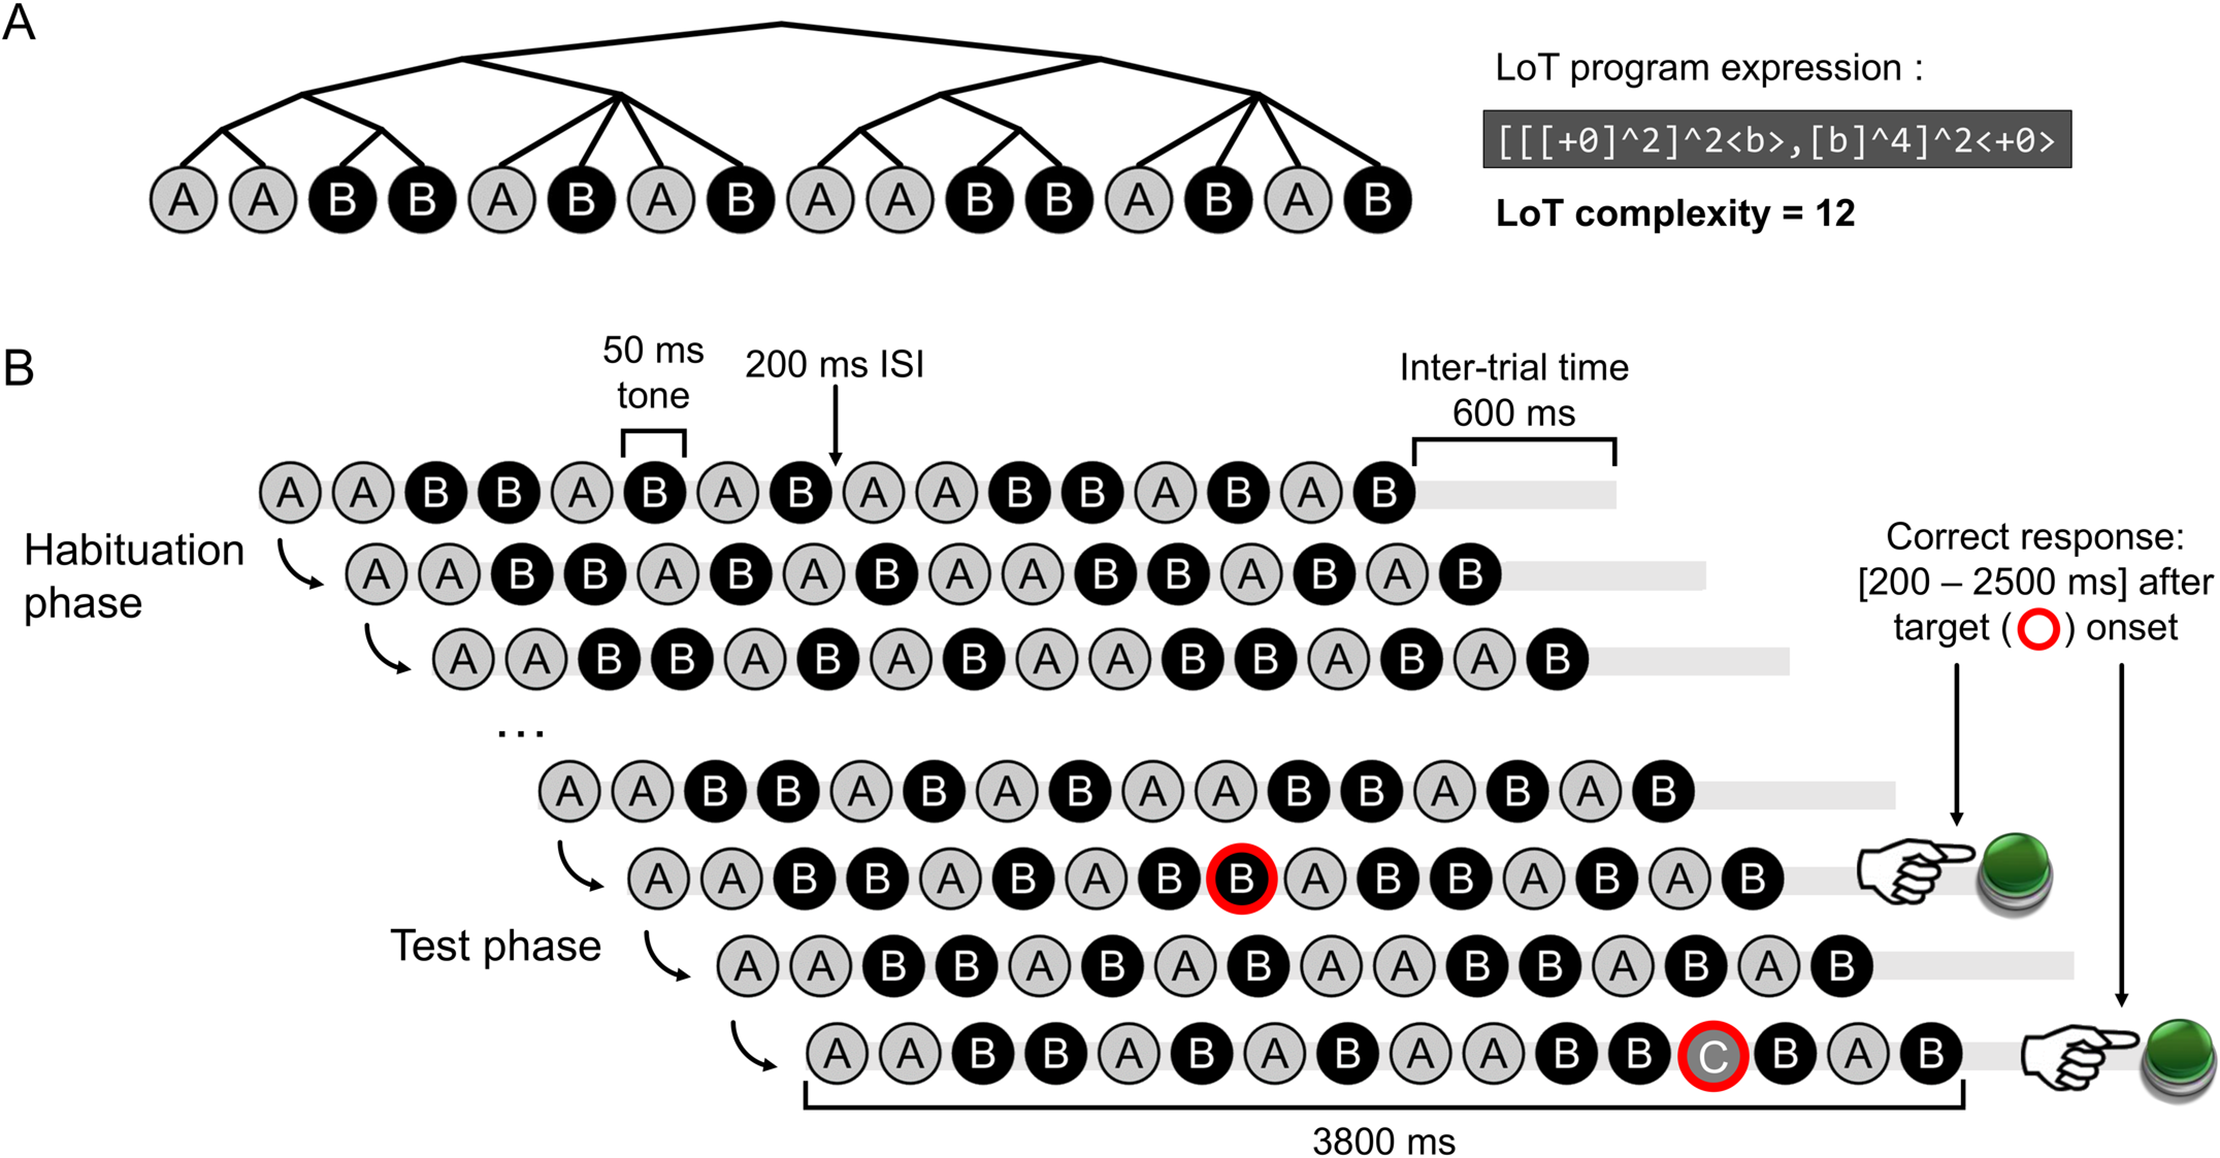
\includegraphics[scale=0.8]{journal.pcbi.1008598.g001.PNG}
     
      \centering
      %Figure 1: (A) Example of a 16-items long sequential pattern, with its shortest representation in the language of thought (i.e. LoT program expression) and the tree-structure derived from this expression (illustrating the hierarchical representation). The LoT complexity of this sequence is also indicated. (B) Experimental design of the violation detection task: a session with the sequence AABBABABAABBABAB is represented, with one example target deviant item (“A” replaced by “B”, at position 9) and one example target super-deviant item (“C” at position 13). Deviants could occur at positions 9, 11, 13 or 15.
     
      \caption{(A) Ejemplo de un patrón de secuencia larga de 16 elementos, con su representación más corta en el LoT (es decir, la expresión del programa LoT) y la estructura de árbol derivada de esta expresión (que ilustra la representación jerárquica). También se indica la complejidad de LoT de esta secuencia. (B) Diseño experimental de la tarea de detección de violaciones: se representa una sesión con la secuencia AABBABABAABBABAB, con un ejemplo de elemento desviado objetivo (A reemplazado por B, en la posición 9) y un ejemplo de elemento super-desviador objetivo (C en la posición 13). Las desviaciones podían ocurrir únicamente en las posiciones 9, 11, 13 o 15}
      \label{PlosBIO-F1}
\end{figure}
\sergio{la figura no está traducida}   

\begin{figure}[t!]
      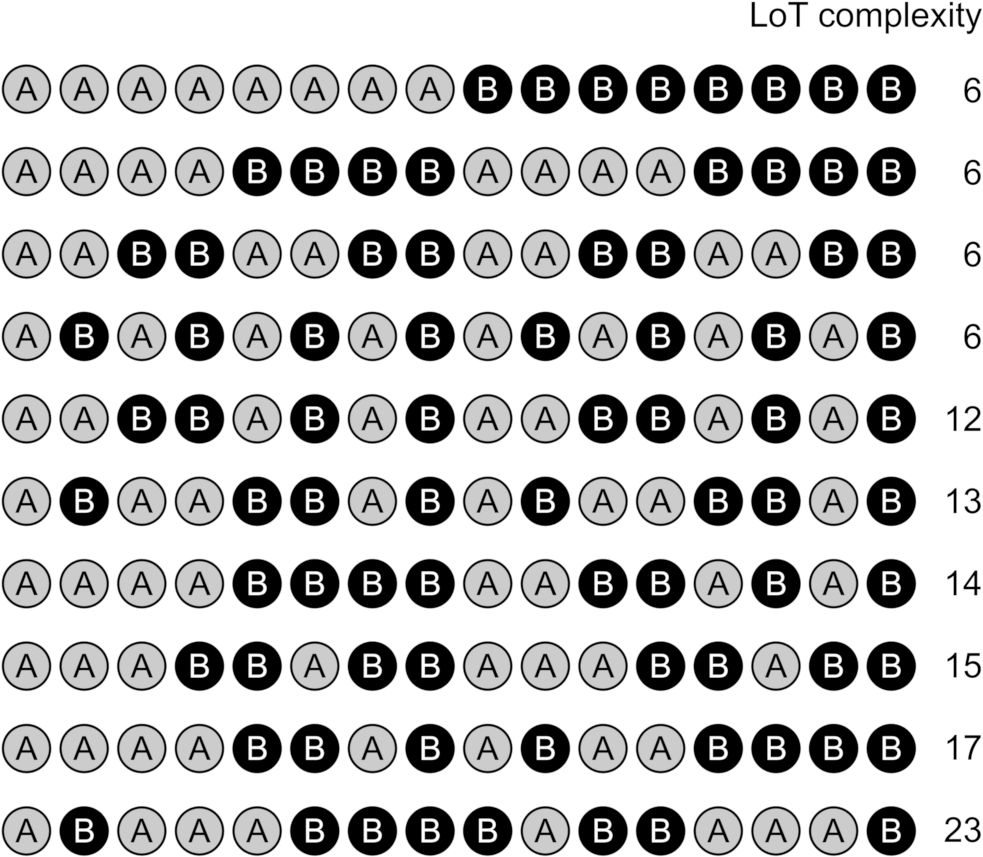
\includegraphics[scale=1]{journal.pcbi.1008598.g002.PNG}
      \centering
      %Ten 16-items long sequential patterns used in experiment 1, with their corresponding LoT complexity value.
      \caption{Diez patrones de secuencias largas de 16 elementos usados en el experimento 1, con su correspondiente valor de complejidad de LoT}
      \label{PlosBIO-F2}
\end{figure}
\sergio{la figura no está traducida}

\subsubsection{Tarea de calificación de complejidad}

%We observed a strong positive linear relationship between average subjective complexity ratings and LoT complexity (entered as a fixed factor in the linear mixed model including participants as the random factor: t(278) = 24.6, p < .0001; Pearson correlation coefficient on the average ratings for each sequence: r = .94) (see Figure 3A). These results indicate that participants were readily able to judge whether a pattern is “more complex” than another, and that the formal language we used to compute sequence complexity is close to how individuals form such complexity judgements.

Se observó una fuerte relación lineal positiva entre la complejidad subjetiva promedio reportada y la complejidad  LoT (introducida como un factor fijo en el modelo mixto lineal que incluye participantes como el factor aleatorio: $t (278) = 24.6, p < 0,0001;$ coeficiente de correlación de Pearson en las calificaciones promedio para cada secuencia: $r = .94$) (ver Figura~\ref{PlosBIO-F3}A ). Estos resultados indican que los participantes pudieron juzgar fácilmente si un patrón es ``más complejo'' que otro, y que el lenguaje formal que usamos para calcular la complejidad de la secuencia se acerca a cómo los individuos forman tales juicios de complejidad.

\subsubsection{Efectos de tipo de desviación y complejidad en la tarea de detección de infracciones}

%We observed a linear relationship of LoT complexity and performance in the violation detection task (using the Linear Integrated Speed-Accuracy Score, LISAS, an integrated measure of response times and error rates, see 87,88). We observed main effects of LoT complexity (t(415.0) = 18.1, p < .0001), deviant type (994 ms for sequence deviants vs. 570 ms for super-deviants; t(414.4) = 18.9, p < .0001) and their interaction (t(414.5) = 11.7, p < .0001). Indeed, the slope of the complexity effect was significantly stronger, by an order of magnitude, for sequence deviants as opposed to super-deviants (respectively +51 ms vs. +5 ms in simple regression, t(16) = 11.7, p < .0001; see Figure 3B, and Fig. S1 for the corresponding results using response times or miss rate instead of LISAS). Nevertheless, separate analyses revealed that LoT complexity was a strong predictor of performance for sequence deviants (t(193.0) = 15.5, p < .0001; r = .98) and also, surprisingly, for super-deviants (t(198.5) = 4.08, p < .0001; r = .72) (Figure 3B). The latter effect on LISAS was however mainly driven by response times, since the average hit-rate for super-deviants was high (96\%) and weakly modulated by LoT complexity (t(200.7) = 2.32, p = .022).

Observamos una relación lineal entre la complejidad LoT y el rendimiento en la tarea de detección de violaciones (utilizando la medida \textit{linear integrated speed-accuracy score} (LISAS), una medida integrada de tiempos de respuesta y tasas de error, ver \cite{f87,f88}). Hemos observado efectos principales de complejidad LoT ($t(415.0) = 18.1 , p <0,0001$), tipo de desviación (994ms para desviaciones de secuencias vs. 570ms para super-desviaciones; $t (414.4) = 18.9 , p < .0001$) y su interacción ( $t(414.5) = 11. 7 , p <.0001$). De hecho, la pendiente del efecto de complejidad fue significativamente más fuerte, en un orden de magnitud, para las desviaciones de secuencia en comparación con las super-desviaciones (respectivamente +51ms frente a +5ms en la regresión lineal, $t(16) = 11.7, p <0.0001$; consulte la Figura~\ref{PlosBIO-F3}B y la Figura~\ref{PlosBIO-S1} para los resultados correspondientes utilizando el tiempo de respuesta o la tasa de errores en lugar de LISAS). Sin embargo, análisis separados revelaron que la complejidad LoT era un fuerte predictor de rendimiento para la desviación de secuencias( $t( 193.0) = 15.5, p <0.0001 ; r = 0.98$) y también, sorprendentemente, para super-desviaciones ($t (198.5) = 4.08, p < .0001 ; r = .72$) (Figura~\ref{PlosBIO-F3}B). El último efecto en LISAS, sin embargo, fue impulsado principalmente por el tiempo de respuesta, ya que la tasa de éxito promedio para super-desviaciones fue alta (96\%) y débilmente modulada por la complejidad LoT ($t(200.7) = 2.32, p =.022$).

%The number of false alarms per sequence (which was 1.99 on average) also increased with sequence LoT complexity (t(214.4)=4.20, p < .0001; r = .74), suggesting here again that the LoT complexity was a good predictor of the quality of sequence encoding.

El número de falsas alarmas por secuencia (que era 1.99 en promedio) también aumentó con la complejidad LoT de la secuencia ($t(214.4)= 4.20, p <0.0001 ; r = 0.74$), lo que sugiere de nuevo que la complejidad LoT es un buen predictor de la calidad de la codificación de secuencias.

%The results of this first experiment with long binary auditory sequences (16 items) thus indicate that the formal language used to describe sequences in a compressed form, based on simple (possibly embedded) rules, is highly relevant to predict (i) how “complex” an auditory sequence is judged by adult participants after having listened to it once and (ii) how difficult it was to learn these sequences in order to detect alterations. 

Los resultados de este primer experimento con secuencias binarias auditivas largas (16 elementos) por lo tanto indican que el lenguaje formal utilizado para describir la secuencia en una forma comprimida, basado en reglas simple con capacidad de ser embebidas, es de gran importancia para predecir (i) cuán ``compleja'' una secuencia auditiva es juzgada por los participantes adultos después de haberla escuchado una vez y (ii) lo difícil que fue aprender estas secuencias para que puedan detectar alteraciones.

%Sequence complexity was expected to have little or no impact on the detection of super-deviants, i.e. high or low pitch tones different from the two tones composing the binary auditory sequence. Our rationale was that such “C” tones were detectable even without any prior knowledge of sequence structure. While performance in detecting super-deviants was much better than for sequence deviants, even for the simplest sequences, a clear relationship between LoT complexity and performance continued to be observed. We see at least two interpretations of this finding. First, there could be an increased attentional cost of having to detect violations in more complex sequences, thus placing subjects in a dual-task setting of having to simultaneously maintain a complex representation in memory and to respond to deviants. Alternatively, the effect could reflect the influence of a top-down prediction system which would use sequence structure to generate predictions of the incoming stimuli. Complex sequences would be less well predicted, and this would in turn affect the speed with which any deviant is detected. We return to this question in the General Discussion.

Se esperaba que la complejidad de la secuencia tenga poco o ningún impacto en la detección de super-desviadaciones, (tonos altos o bajos diferentes de los dos tonos que componen la secuencia auditiva binaria). Nuestro razonamiento fue que esos tonos C eran detectables incluso sin ningún conocimiento previo de la estructura de la secuencia. Si bien el rendimiento en la detección de super-desviaciones fue mucho mejor que para las desviaciones de secuencia, incluso para las secuencias más simples, se siguió observando una relación clara entre la complejidad LoT y el rendimiento. Vemos al menos dos interpretaciones de este hallazgo. Primero, podría haber un mayor costo de atención de tener que detectar violaciones en secuencias más complejas, colocando así a los sujetos en un entorno de una doble tarea de tener que mantener simultáneamente una representación compleja en la memoria y responder a las desviaciones. Alternativamente, el efecto podría reflejar la influencia de un sistema de predicción de arriba hacia abajo que usaría la estructura de secuencia para generar predicciones de los estímulos entrantes. Las secuencias complejas se predecirían peor y esto, a su vez, afectaría la velocidad con la que se detecta cualquier desviación. Volvemos a esta cuestión en la \ref{chapter:BOI-GeneralDiscusion}.

\subsubsection{Efectos de sorpresa}

%Many prior experiments, using either or both behavior and brain-imaging measures, have shown that individuals constantly entertain predictions about future observations using probabilistic knowledge based on past observations (e.g. 19,20). In order to test whether task performance could be explained by a learning transition probabilities (surprise) only, or also truly implied an encoding of sequence structure, we compared a mixed model (with participants as a random effect) including fixed effects of both LoT complexity and surprise (averaged across the 4 possible positions of deviants in a given sequence) with a null model including only surprise. The effect of surprise in the null model with surprise alone) was significant (t(193.0) = 5.31, p < .0001). However, a likelihood ratio test showed that adding LoT complexity significantly improved the goodness of fit: χ²(1) = 130.9, p < .0001. Adding a “period” factor (i.e. period values were 2, 4, 8 or 16) as a third fixed effect did not improve the model fit (χ2(1) = 1.23, p = .267), confirming the prediction that the four included AnBn patterns have the same psychological complexity, and suggesting that this information is already captured by LoT complexity. Adding the interaction between surprise and LoT complexity did not improve goodness of fit either (χ2(1) = 2.50, p = .114). As reported in Table 1, the LoT complexity fixed effect was significant in the final full model (t(192.4) = 13.6, p < .0001), but not the surprise fixed effect (t(191.8) = 0.60, p = .55). The absence of a significant effect of surprise once sequence complexity is taken into account reflects the existence of a correlation between the two measures (r = –.54): biased transition probabilities in less complex sequences tending to make deviants more easily surprising. It also shows that when these two slightly colinear factors are included, LoT is more effective than surprise at describing the variance of the data.

Muchos experimentos previos, utilizando alguna o ambas medidas de comportamiento y de imagen cerebral, han demostrado que los individuos constantemente generan predicciones de futuras observaciones usando el conocimiento probabilístico basado en observaciones anteriores (por ejemplo, \cite{f19,f20}). Para probar si el desempeño de la tarea podría explicarse sólo como un aprendizaje de la transición de probabilidad (sorpresa), o si también implicaba realmente una codificación de la estructura de la secuencia, comparamos un modelo mixto (con participantes como un efecto aleatorio) que incluye efectos fijos de complejidad LoT y sorpresa (promediada entre las 4 posibles posiciones de las desviaciones en una secuencia dada) con un modelo nulo que incluye sólo la sorpresa. El efecto de sorpresa en el modelo nulo con sorpresa sola) fue significativo ($t(193.0) = 5.31, p < .0001$). Sin embargo, una prueba de razón de verosimilitud mostró que agregar la complejidad LoT mejoraba significativamente la bondad de ajuste: $\chi^2(1) = 130.9, p <.0001$. Agregar un factor de ``período'' (los valores del período fueron 2, 4, 8 o 16) como un tercer efecto fijo no mejoró el ajuste del modelo ($\chi^2(1) = 1.23, p =.267$), lo que confirma la predicción de que los cuatro patrones $A^n B^n$ incluidos tienen la misma complejidad subjetiva, y sugiere que esta información ya está capturada por la complejidad LoT. La adición de la interacción entre la sorpresa y la complejidad LoT tampoco mejoró la bondad del ajuste ($\chi^2(1) = 2.50, p =.114$). Como se informa en la Tabla~\ref{PlosBIO-T1} , el efecto fijo de la complejidad LoT fue significativo en el modelo completo final ($t(192.4) = 13.6, p <.0001$), pero no el efecto fijo de la sorpresa ($t ( 191.8) = 0.60, p = .55$). La ausencia de un efecto de sorpresa significativo una vez que se tiene en cuenta la complejidad de la secuencia refleja la existencia de una correlación entre las dos medidas ( $r = - . 54$): probabilidades de transición sesgadas en secuencias menos complejas tienden a hacer que las desviaciones sean más fácilmente sorprendentes. También muestra que cuando se incluyen dos factores con una pequeña colinealidad, LoT es más eficaz que la sorpresa en la descripción de la varianza de los datos.

%As our choice of attributing an arbitrary padding value (0.01) to deviant transitions events with zero probability when computing surprise may have biased the results, we recomputed the LISAS and average surprise while excluding all such trials (i.e. all deviant positions in the (AB)8 pattern, 3 out of 4 deviant positions in the A8B8 pattern). Here again, a likelihood ratio test showed that the goodness of fit increased significantly when adding LoT complexity to a null model containing only surprise (χ²(1) = 116.3, p < .0001). However, both complexity (t(165.5) = 12.9, p < .0001) and surprise (t(165.8) = 3.82, p < .0001) were significant with this subset of the data.

Como nuestra elección de atribuir un arbitraria valor de relleno (0.01) a los eventos de transición de desviaciones con probabilidad cero al calcular la sorpresa puede haber sesgado los resultados, recomputamos la medida LISAS y la media de la sorpresa excluyendo todos esos ensayos (es decir, todas las posiciones de desviación en el patrón $(AB)^8$ y 3 de 4 posiciones de desviación en el patrón $A^8 B^8$) . Aquí nuevamente, una prueba de razón de verosimilitud mostró que la calidad del ajuste aumentó significativamente cuando se agregó la complejidad LoT a un modelo nulo que sólo contenía sorpresa ($\chi^2(1) = 116.3, p <.0001$). Sin embargo, tanto la complejidad ($t ( 165.5) = 12.9, p <.0001$) como la sorpresa ( t ($165.8) = 3.82, p <.0001$) fueron significativas con este subconjunto de datos. \sergio{entender efecto de relleno explicado}

%In conclusion, the strong complexity effects observed here indicated that participants used some form of compression of information to encode the sequence and perform the task over and above simply learning statistical trends. Although no instruction was given in that sense, this strategy may be needed in order to deal with a difficult, memory-demanding task. Indeed, at the maximum level of complexity used, performance in violation detection was very low (the violation detection rate dropped to 41% for sequence deviants).

En conclusión, los fuertes efectos de complejidad observados indicaron que los participantes usan alguna forma de compresión de la información para codificar la secuencia y realizar la tarea más allá de simplemente aprender tendencias estadísticas de los elementos. Aunque no se dio ninguna instrucción en ese sentido, esta estrategia puede ser necesaria para hacer frente a una tarea difícil que exige memoria. De hecho, en el nivel máximo de complejidad utilizado, el rendimiento en la detección de violaciones fue muy bajo (la tasa de detección de violaciones se redujo al 41\% para las desviaciones de secuencias).

%In the subsequent experiments, we asked whether similar complexity effects emerged in the same paradigm but with shorter sequences. That is, when the sequence can be more easily encoded and stored “as a whole”, without necessarily requiring a re-encoding in a more abstract, compressed form. In these less demanding conditions, it can be expected that the spontaneous encoding of transitions probabilities between items will play a more important role in the detection of violations.

En los experimentos posteriores, nos preguntamos si los efectos de complejidad similares pueden ser vistos en el mismo paradigma, pero con secuencias más cortas. Es decir, cuando la secuencia se puede codificar y almacenar más fácilmente ``en su conjunto'', sin que se requiera necesariamente una recodificación en una forma más abstracta o comprimido. En estas condiciones menos exigentes, se puede esperar que la codificación espontánea de las probabilidades de transición entre elementos juegue un papel más importante en la detección de violaciones.

\begin{figure}[t!]
      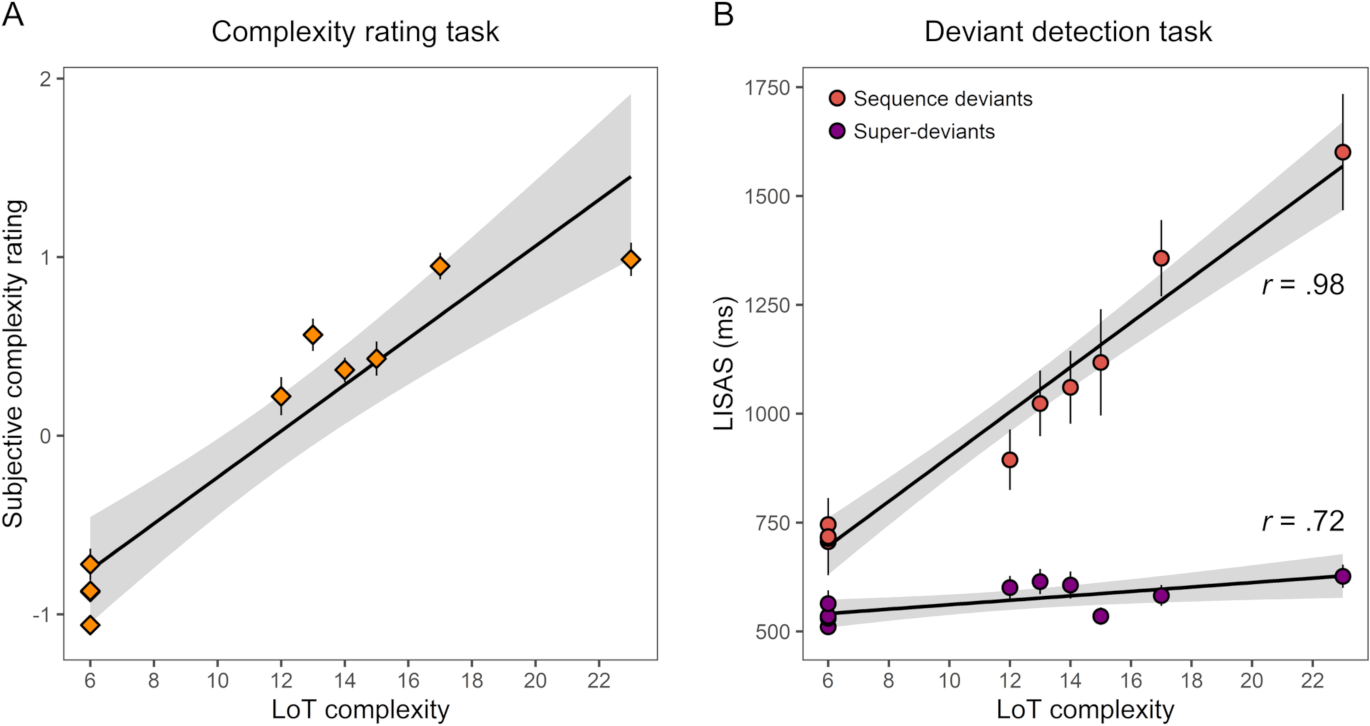
\includegraphics[scale=1]{journal.pcbi.1008598.g003.PNG}
      \centering
      %Linear relationship between LoT complexity and subjective and objective measures obtained in experiment 1 with ten 16-items long auditory sequences (with 95% confidence intervals bands in gray). The Pearson correlation coefficient (r)  is indicated. Each marker represents the group-average for a given sequence. Error bars represent SEM across participants. (A) LoT complexity vs. subjective complexity ratings. (B) LoT complexity vs. performance in the violation detection task (Linear Integrated Speed-Accuracy Score), for sequence deviants and super-deviants.
      \caption{Relación lineal entre la complejidad LoT y las medidas subjetivas y objetivas obtenidas en el experimento 1 con diez secuencias auditivas largas de 16 elementos (intervalos de confianza del 95\% en gris). El coeficiente de correlación de Pearson (r) aparece indicado. Cada marcador representa el promedio del para una determinada secuencia. Las barras de error representan el s.e.m. entre los participantes. (A) Clasificación de complejidad LoT frente a complejidad subjetiva. (B) Complejidad LoT frente a rendimiento en la tarea de detección de violaciones (medida integrada de tiempos de respuesta y tasas de error, LISAS), para desviaciones de secuencia y super-desviaciones.}
      \label{PlosBIO-F3}
\end{figure}
\sergio{la figura no está traducida}

\begin{table}[]
\centering
\begin{tabular}{lccccc}
\multicolumn{6}{l}{\textbf{Experimento 1} (secuencias de 16 elementos, excluyendo super-desviados)}                                                    \\ \hline
\textit{Predictores}          & \textit{Estimados}   & \textit{Std. Error}  & \textit{Valor t}     & \textit{IC del 95\%} & \textit{pag}              \\ \hline
(Interceptar)                 & 356,90               & 80,51                & 4.43                 & 199,5 - 514,3        & \textbf{\textless{}.0001} \\
Complejidad                   & 52.15                & 3,84                 & 13.60                & 44,6 - 59,7          & \textbf{\textless{}.0001} \\
Sorpresa                      & 6,77                 & 11.31                & 0,60                 & -15,4 - 28,9         & .55                       \\ \hline
\multicolumn{1}{c}{}          & \multicolumn{1}{l}{} &                      &                      &                      &                           \\
\multicolumn{6}{l}{\textbf{Experimento 2} (secuencias de 12 elementos, excluyendo super-desviados)}                                                    \\ \hline
\textit{Predictores}          & \textit{Estimados}   & \textit{Std. Error}  & \textit{Valor t}     & \textit{IC del 95\%} & \textit{pag}              \\ \hline
(Interceptar)                 & 852,38               & 124,91               & 6,82                 & 608,5 - 1096,2       & \textbf{\textless{}.0001} \\
Complejidad                   & 24,21                & 6.29                 & 3,85                 & 11,9 - 36,5          & \textbf{\textless{}.0002} \\
Sorpresa                      & -43,13               & 21.06                & -2.05                & -84,4 - -1,9         & \textbf{\textless{}.05}   \\ \hline
\textbf{}                     & \multicolumn{1}{l}{} & \multicolumn{1}{l}{} & \multicolumn{1}{l}{} & \multicolumn{1}{l}{} & \multicolumn{1}{l}{}      \\
\multicolumn{6}{l}{\textbf{Experimento 3} (secuencias de 8 elementos)}                                                                                \\ \hline
\textit{Predictores}          & \textit{Estimados}   & \textit{Std. Error}  & \textit{Valor t}     & \textit{IC del 95\%} & \textit{pag}              \\ \hline
(Interceptar)                 & 852.40               & 73,39                & 11,62                & 707,8 - 997          & \textbf{\textless{}.0001} \\
Complejidad                   & 10,75                & 3,49                 & 3,08                 & 3,9 - 17,6           & \textbf{\textless{}.003}  \\
Sorpresa                      & -32,37               & 5.60                 & -5,78                & -43,3 - -21,4        & \textbf{\textless{}.0001} \\ \hline
\multicolumn{1}{c}{\textbf{}} & \multicolumn{1}{l}{} & \multicolumn{1}{l}{} & \multicolumn{1}{l}{} & \multicolumn{1}{l}{} & \multicolumn{1}{l}{}      \\
\multicolumn{6}{l}{\textbf{Experimento 4} (secuencias de 6 elementos, secuencia 'AAAAAA' excluida)}                                                   \\ \hline
\textit{Predictores}          & \textit{Estimados}   & \textit{Std. Error}  & \textit{Valor t}     & \textit{IC del 95\%} & \textit{pag}              \\ \hline
(Interceptar)                 & 751,6                & 47,5                 & 15,8                 & 658,8 - 844,5        & \textbf{\textless{}.0001} \\
Complejidad                   & 1.4                  & 4.4                  & 0,3                  & -7,2 - 9,9           & .75                       \\
Sorpresa                      & -15,3                & 3.8                  & -4,1                 & -22,7 - -7,9         & \textbf{\textless{}.0001} \\ \hline
\multicolumn{1}{c}{\textbf{}} & \multicolumn{1}{l}{} & \multicolumn{1}{l}{} & \multicolumn{1}{l}{} & \multicolumn{1}{l}{} & \multicolumn{1}{l}{}      \\
\multicolumn{6}{l}{\textbf{Experimento 5} (secuencias de 8 ítems, auditivo y visual)}                                                                 \\ \hline
\textit{Predictores}          & \textit{Estimados}   & \textit{Std. Error}  & \textit{Valor t}     & \textit{IC del 95\%} & \textit{pag}              \\ \hline
(Interceptar)                 & 645,1                & 92,2                 & 7.0                  & 464,4 - 825,9        & \textbf{\textless{}.0001} \\
Complejidad                   & 25,2                 & 25,2                 & 4.4                  & 14 - 36,4            & \textbf{\textless{}.0001} \\
Sorpresa                      & -36,7                & 8.1                  & -4,5                 & -52,5 - -20,8        & \textbf{\textless{}.0001} \\
Modalidad (visual)            & 337,0                & 337,0                & 14,2                 & 290,7 - 383,3        & \textbf{\textless{}.0001} \\ \hline
\end{tabular}
\caption{Efectos fijos en los modelos lineales mixtos, separados para cada experimento}
\label{PlosBIO-T1}
\end{table}

\section{Experimento 2 : secuencias auditivas con 12 elementos}

%In order to test whether the previous results could be replicated with shorter sequences, in experiment 2, the same tasks and procedure were used (with a different group of participants), this time using twelve sequences of twelve items (spanning a large range of complexities, see Figure 4).

Para probar si los resultados anteriores podían replicarse con secuencias más cortas, en el experimento 2, se utilizaron las mismas tareas y el mismo procedimiento (con un grupo diferente de participantes), pero esta vez usando doce secuencias de doce elementos (que abarcan una amplia gama de complejidades, vea la Figura~\ref{PlosBIO-F4}).

\begin{figure}[t!]
      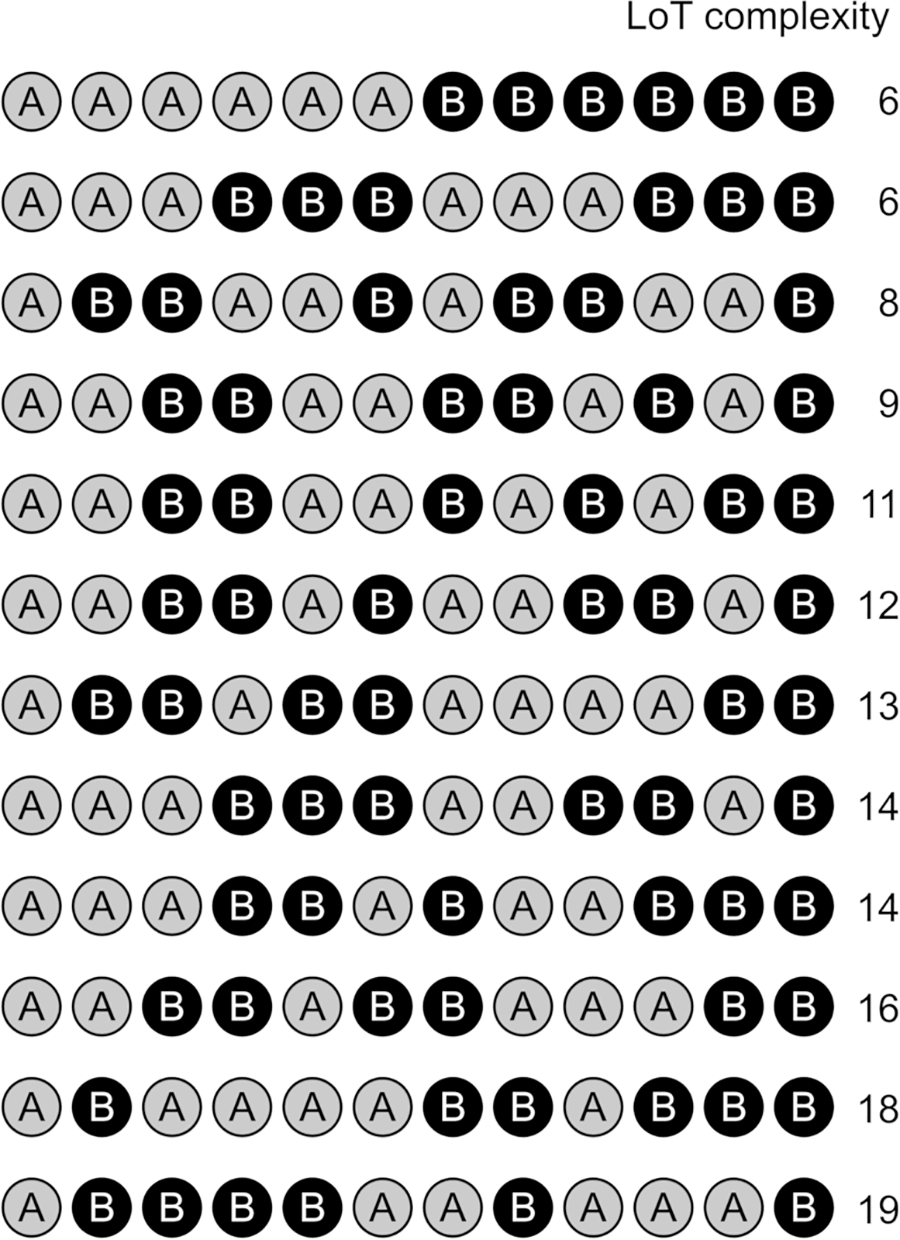
\includegraphics[scale=1]{journal.pcbi.1008598.g004.PNG}
      \centering
      %Twelve 12-item sequences used in experiment 2, with their corresponding LoT complexity value (in bits).
      \caption{Doce secuencias de 12 elementos utilizadas en el experimento 2, con su correspondiente valor de complejidad LoT (en bits)}
      \label{PlosBIO-F4}
\end{figure}
\sergio{la figura no está traducida}

\subsubsection{Tarea de calificación de complejidad}

%A positive linear relationship was found between subjective complexity ratings and LoT complexity (t(238) = 6.81 p < .0001, r = .61). The correlation of the average score per sequence with LoT complexity was however less strong than what was observed in the previous experiment with 16-items long sequences (r = .61, see Figure 5A). Subjective complexity was clearly underestimated for one specific sequence (ABBAABABBAAB, predicted complexity of 8), which is confirmed by an inspection of the residuals of the regression (residual 1.99 SD above average for this sequence).

Se encontró una relación lineal positiva entre los reportes de complejidad subjetiva y la complejidad LoT ($t(238) = 6.81 p <.0001 , r = .61$). La correlación de la complejidad subjetiva media por secuencia con la complejidad LoT era, sin embargo, menos fuerte que lo observado en el experimento anterior con 16 secuencias largas de 16 elementos ($r = .61$, ver Figura~\ref{PlosBIO-F4}A). La complejidad subjetiva estaba claramente subestimada para una secuencia específica (ABBAABABBAAB, con una complejidad predicha de 8), lo cual se confirma con una inspección de los residuos de la regresión (residual 1.99 SD por encima del promedio para esta secuencia).

%Deviant type and complexity effects in the violation detection task
\subsubsection{Tipos de desviaciones y efectos de la complejidad en la tarea de detección de violaciones}

%Regarding the violation detection task, main effects of LoT complexity (t(431.1) = 6.43, p < .0001) and deviant type (1078 ms for sequence deviants vs. 545 ms for super-deviants; t(431.0) = 19.3, p < .0001) were observed, as well as their interaction (t(431.1) = 3.48, p < .001). The slope of the complexity effect appeared indeed slightly stronger for sequence deviants as opposed to super-deviants, although the comparison did not reach significance when using simple linear regressions with averaged LISAS per sequence (slopes of respectively +30 ms vs. +7 ms, t(20) = 1.87, p = .077; see Figure 5B, and Fig. S2 for the corresponding results with RTs and miss rates instead of LISAS). Separated analyses revealed that the effect of LoT complexity was significant in analyses restricted to either sequence deviants (t(205.1) = 5.78, p < .0001; r = .63), or super-deviants (t(208.0) = 2.88, p = .005; r = .59) only. The number of false alarms per sequence (3.88 on average) was also significantly predicted by the LoT complexity of the sequence (t(208.0) = 3.50, p < .001; r = .56).

Con respecto a la tarea de detección de violaciones, los principales efectos de la complejidad LoT ($t ( 431.1) = 6.43, p <.0001$) y el tipo de desviación (1078 ms para desviaciones de secuencia vs 545 ms para super-desviaciones; $t ( 431.0) = 19.3, p <.0001$), así como su interacción ($t ( 431.1) = 3.48, p <.001$). La pendiente del efecto de complejidad apareció de hecho ligeramente más fuerte para las desviaciones de secuencia en comparación con las super-desviaciones, aunque la comparación no fue significativa cuando se usaron regresiones lineales simples con LISAS promediado por secuencia ( pendientes de +30 ms frente a +7 ms, respectivamente , $t (20) = 1.87, p = .077$; consulte la Figura~\ref{PlosBIO-F5}B y la Figura~\ref{PlosBIO-S2} para obtener los resultados correspondientes con tiempo de respuesta y tasas de error en lugar de LISAS). Los análisis separados revelaron que el efecto de la complejidad LoT fue significativo en los análisis restringidos a secuencias con desviaciones ($t ( 205.1) = 5.78, p <.0001; r = .63$), o super-desviaciones ($t ( 208.0) = 2.88, p = .005; r = .59$) solamente . El número de falsas alarmas por secuencia (3.88 en promedio) también fue predicho significativamente por la complejidad LoT de la secuencia ($t ( 208,0) = 3,50, p <.001; r = .56$).

%As in the complexity rating task, although the overall correlation was high, a noticeable deviation between predicted complexity and observed performance was present for some of the sequences. In fact, the correlation profiles observed in the Figure 5A and 5B suggest that the psychological complexity of the pattern, as indexed by subjective rating or violation detection task performance, might have been, for some sequences, consistently overestimated or underestimated by the LoT across both tasks (the largest residual in the regression with the sequence deviants, 1.50 SD above average, corresponded to the same sequence identified by complexity ratings: ABBAABABBAAB). To further test this idea, we computed the correlation between the residuals of both linear regressions. The correlation was significant (t(10) = 4.02; p = .003), indicating that even after regressing out the effect of LoT complexity, the data from both experiments remained correlated with each other, and thus that, although the proposed LoT is a good predictor, it does not fully account for all details of the psychological complexity of patterns. One attempt to address the limitations of the language, by proposing a modification of it, is reported in the Further analysis section.

Al igual que en la tarea de calificación de complejidad, aunque la correlación general fue alta, hubo una desviación notable entre la complejidad predicha y el rendimiento observado para algunas de las secuencias. De hecho, los perfiles de correlación observados en la Figura~\ref{PlosBIO-F5}A y la Figura~\ref{PlosBIO-F5}B sugieren que la complejidad psicológica del patrón, según lo indexado por la calificación subjetiva o el desempeño de la tarea de detección de violaciones, podría haber sido para algunas secuencias constantemente sobrestimado o subestimado por el LoT en ambas tareas (el residuo más grande en la regresión con las desviaciones de secuencia, 1.50 SD por encima del promedio, correspondió a la misma secuencia identificada por la clasificación de complejidad subjetiva: ABBAABABBAAB ). Para probar más esta idea, calculamos la correlación entre los residuos de ambas regresiones lineales. La correlación fue significativa ($t (10) = 4.02; p  = .003$), lo que indica que -incluso después de hacer una regresión del efecto de la complejidad LoT- los datos de ambos experimentos permanecieron correlacionados entre sí y, por lo tanto, aunque el LoT propuesto es un buen predictor, no explica por completo todos los detalles de la complejidad psicológica de los patrones. Un intento de abordar las limitaciones del lenguaje, proponiendo una modificación, se informa en la sección \ref{PlosBIO-AnalisisAdiocional}.

\begin{figure}[t!]
      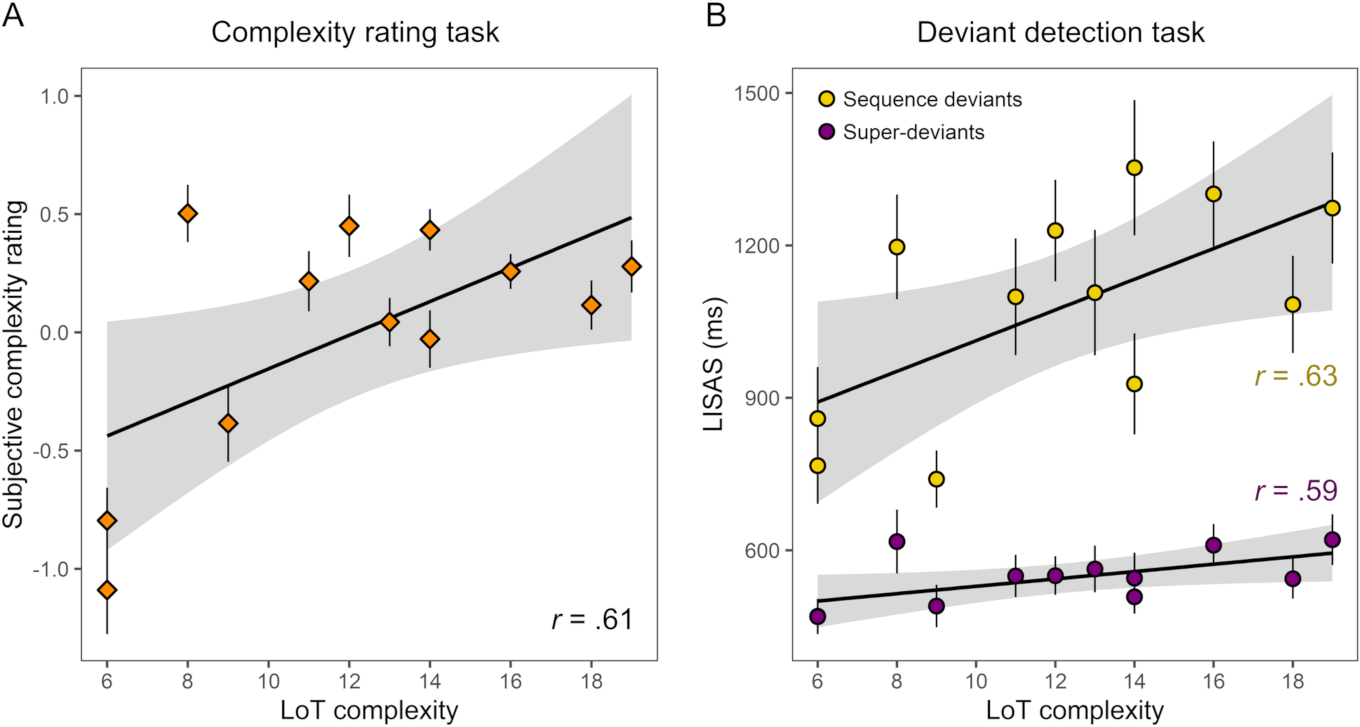
\includegraphics[scale=1]{journal.pcbi.1008598.g005.PNG}
      \centering
      %Linear relationship between LoT complexity and scores obtained in the two tasks of experiment 2 with 12-item auditory sequences (with 95% confidence intervals bands in gray). Same format as Figure 3.
      \caption{Relación lineal entre la complejidad LoT y las puntuaciones obtenidas en las dos tareas del experimento 2 con secuencias auditivas de 12 elementos (con bandas de intervalos de confianza del 95\% en gris). Mismo formato que la Figura~\ref{PlosBIO-F3}}
      \label{PlosBIO-F5}
\end{figure}
\sergio{la figura no está traducida}

\subsubsection{Efectos de sorpresa}
%A comparison of mixed models (with participants as a random effect) showed that, compared to a null model including surprise as the sole predictor (null model; in which the main predictor was significant: t(205.0) = 4.67, p < .0001), a model additionally including LoT complexity (full model) fitted the data better (likelihood ratio test : χ²(1) = 14.4, p < .001). Both fixed effects were significant in the full model: LoT complexity (t(204.1) = 3.85, p < .0001), as well as surprise (t(204.0) = 2.05, p = .042) (see Table 1). Although we observed, contrary in the previous experiment, an effect of statistical learning (indexed by the level of surprise of deviant items), it was only barely statistically significant.

Una comparación de modelos mixtos (con participantes como el efecto aleatorio) mostró que, en comparación con un modelo nulo que incluye la sorpresa como único predictor (modelo nulo en el que el predictor principal fue significativo: $t (205,0) = 4,67, p <0,0001$), un modelo que incluye adicionalmente la complejidad LoT (modelo completo) explica mejor los datos (prueba de razón de verosimilitud: $\chi^2(1) = 14.4, p <.001$). Ambos efectos fijos fueron significativos en el modelo completo: complejidad LoT ($t ( 204.1) = 3.85 , p <.0001$) , así como la sorpresa ($t ( 204.0 ) = 2.05 , p= .042$) (ver Tabla~\ref{PlosBIO-T1}). Aunque hemos observado, al contrario que en el experimento anterior, un efecto de aprendizaje estadístico (indexado por el nivel de la sorpresa del elemento desviado), que era sólo apenas estadísticamente significativo.

\subsection{Experimento 3 y 4: secuencias auditivas con 6 u 8 elementos}

%Results of experiments 1 and 2 showed that our sequence complexity metric was well correlated with behavior, suggesting that our formal language provided a good approximation of the internal language of thought that humans use to encode a sequence in memory a compressed from. These results were however obtained with a restricted set of sequences, which were long enough to promote hierarchical representations based on the repetition and alternation operations, and to probe a large range of complexity values. The main objective of experiments 3 (with 35 8-items long sequences, see Fig. S3) and 4 (with 32 6-items long sequences, see Fig. S4) was to test whether the effect of complexity observed in the first two experiments could be generalized to a larger set of shorter sequences, where we could examine more gradual variations in complexity. Given that human working memory is thought to store and maintain 4 to 7 items without compression, or with a minimal chunking process (25,29), we expected the predictive power of our language to be reduced compared with previous experiments with longer sequences, while the effects of transition probabilities would increase. The same violation detection paradigm was used. No subjective complexity ratings were collected (given the larger number of individual sequences compared to the previous experiments). 

Los resultados de los experimentos 1 y 2 mostraron que nuestra métrica de complejidad de secuencia se correlacionaba bien con el comportamiento, lo que sugiere que nuestro lenguaje formal proporcionó una buena aproximación del lenguaje interno del pensamiento que los humanos usan para codificar una secuencia comprimida en la memoria. Sin embargo, estos resultados se obtuvieron con un conjunto restringido de secuencias, que eran lo suficientemente largas para promover representaciones jerárquicas basadas en las operaciones de repetición y alternancia, y para probar una amplia gama de valores de complejidad. El objetivo principal del experimento 3 (con 35 secuencias largas de 8 elementos, ver Figura~\ref{PlosBIO-S3}) y del experimento 4 (con 32 secuencias largas de 6 elementos, ver Figura~\ref{PlosBIO-S4}) fue probar si el efecto de la complejidad observado en los dos primeros experimento podría ser generalizados a un conjunto más amplio de secuencias más cortas, en donde podamos examinar variaciones más graduales de la complejidad. Dado que la memoria de trabajo humana está pensada para almacenar y mantener de 4 a 7 elementos sin compresión, o con un proceso de agrupamiento mínimo (\cite{f25,f29}) , esperamos que le poder predictivo de nuestro LoT se reduzca en comparación con los experimentos anteriores realizados con secuencias más largas, mientras que los efectos de las transiciones de probabilidad aumenten. Utilizamos en estos experimentos el mismo paradigma de detección de violaciones. No se recopilaron calificaciones de complejidad subjetiva (dado el mayor número de secuencias individuales en comparación con los experimentos anteriores).

%Here again, we tested (using mixed models) whether surprise suffices to explain the variance in performance or if a significant proportion of variance remained yet to be explained by sequence complexity (all models included participants as a random effect). In experiment 3 (8-items sequences, N = 35), goodness of fit improved when LoT complexity was included in the model (χ²(1) = 9.47, p = .002). Both fixed effects were significant in the full model: LoT complexity (t(1042.0) = 3.08, p = .002; see Figure 6A, and Fig. S5), as well as surprise (t(1042.0) = 5.78, p < .0001) (see Table 1). Note that the surprise fixed effect was already highly significant in the null model (t(1043.0) = 8.72, p < .0001).

Una vez más, hemos probado (utilizando modelos mixtos) si es suficiente la sorpresa para explicar la variación en el rendimiento o si una proporción significativa de la varianza se mantuvo aún para ser explicada por la complejidad de la secuencia (todos los modelos incluyen los participantes como efecto aleatorio). En el experimento 3 (secuencias de 8 elementos, N = 35), la calidad del ajuste mejoró cuando se incluyó la complejidad LoT en el modelo ($\chi^2(1) = 9.47, p= .002$). Ambos efectos fijos fueron significativos en el modelo completo: complejidad LoT ( $t ( 1042.0) = 3.08, p <=.002$; ver Figura~\ref{PlosBIO-F6}A y Figura~\ref{PlosBIO-S5}), así como la sorpresa ($t ( 1042.0) = 5.78, p <.0001$) (ver Tabla~\ref{PlosBIO-T1}). Tenga en cuenta que el efecto fijo de la sorpresa ya era muy significativo en el modelo nulo ($t (1043.0) = 8.72, p <.0001$).

%Similarly, in experiment 4 (6-items sequences, N = 32), goodness of fit improved when LoT complexity was included in the surprise-only null model (χ²(1) = 6.20, p = .013) with both fixed effects significant in the full model (LoT complexity: t(649.00) = 2.49, p = .013; see Figure 6B, and Fig. S6), and surprise (t(649.0) = 5.48, p < .0001). The surprise fixed effect was here again already highly significant in the null model (t(650.0) = 6.78, p < .0001). However, one sequence appeared as an outlier in this experiment, with an average LISAS 3.9 SD below the average of all sequences (i.e. indicating a much better performance): the AAAAAA sequence. In this case, performing the task requires no sequence learning, but merely remembering the identity of the A sound, and violation detection is therefore similar to a classic oddball paradigm. When this sequence was removed from the dataset (it was also excluded from further analyses), the inclusion of the complexity fixed factor did no longer improved model goodness of fit (χ²(1) = 0.10, p = .752). Indeed, the LoT complexity fixed effect was not significant in the full model (t(628.0) = 0.32, p = .752), as opposed to the surprise fixed effect (t(628.0) = 4.07, p < .0001) (see Table 1). No improvement in model fit was found when including the interaction between complexity and surprise (χ²(1) = 0.08 in experiment 3, χ²(1) = 0.34 in experiment 4).

Del mismo modo, en el experimento 4 (secuencias de 6 elementos, N = 32), la calidad del ajuste mejoró cuando la complejidad LoT se incluyó en el modelo nulo con la sorpresa como único factor ($\chi^2(1) = 6.20 , p= .013$) con ambos efectos fijos significativos en el modelo completo (complejidad LoT: $t ( 649.00) = 2.49, p= .013$; ver Figura~\ref{PlosBIO-F6}B y Figura~\ref{PlosBIO-S6}) y sorpresa ($t ( 649.0) = 5.4 8, p <.0001$). El efecto fijo de la sorpresa fue ya aquí otra vez altamente significativo en el modelo nulo ($t (650.0) = 6.78 , p <.0001$). Sin embargo, una secuencia apareció como un valor atípico en este experimento, con un LISAS 3,9 SD promedio por debajo del promedio de todas las secuencias (es decir, lo que indica un rendimiento mucho mejor): la secuencia AAAAAA. En este caso, realizar la tarea no requiere un aprendizaje de secuencia, sino simplemente recordar la identidad del sonido A, y la detección de la violación es, por lo tanto, similar a un paradigma clásico de bichos raros (\textit{oddball}). Cuando esta secuencia se eliminó del conjunto de datos (también se excluyó de análisis posteriores), la inclusión del factor fijo de complejidad ya no mejoró la bondad de ajuste del modelo ($\chi^2 (1) = 0.10, p =.752$). De hecho, el efecto fijo de la complejidad LoT no fue significativo en el modelo completo ($t ( 628.0) = 0.32, p =.752$) , a diferencia del efecto fijo de la sorpresa ($t ( 628.0) = 4.07, p <.0001$) (ver Tabla~\ref{PlosBIO-T1}). No se encontró ninguna mejora en el ajuste del modelo al incluir la interacción entre complejidad y sorpresa ($\chi^2(1) = 0.08$ en el experimento 3, $\chi^2(1) = 0.34$ en el experimento 4).

%Beside the effect of complexity, the strong effect of surprise in both experiments indicates that participants were quicker and more likely to detect a deviant when it violated statistical regularities characterizing the auditory sequence being repeatedly played. This is consistent with the idea that humans spontaneously encode the probabilities associated with events and react to surprising events depending on their level of predictability (19,21).

Además del efecto de la complejidad, el fuerte efecto de la sorpresa en ambos experimentos indica que los participantes fueron más rápidos y más propensos a detectar un desviado cuando violaba las regularidades estadísticas que caracterizan la secuencia auditiva que se reproduce repetidamente. Esto es consistente con la idea de que el ser humano codifica de manera espontánea las probabilidades asociadas con eventos y reacciona a los eventos sorprendentes en función de su nivel de previsibilidad \cite{f19,f22}.

%The number of false alarms was low in the present experiments (0.91 per sequence on average in experiment 3, 0.60 in experiment 4). It was slightly related to sequence complexity in experiment 3 t(1048) = 2.19, p = .029) but not in experiment 4 t(650.0) = 0.29, p = .77).

El número de falsas alarmas fue bajo en los presentes experimentos (0.91 por secuencia en promedio en el experimento 3, 0.60 en el experimento 4). Estuvo levemente relacionado con la complejidad de la secuencia en el experimento 3 ($t ( 1048 ) = 2.19 , p=.029$) pero no en el experimento 4 ($t ( 650.0 ) = 0. 29 , p =. 77$).

%Compared to the previous experiment with lengths 12 and 16, it was expected here, with sequences of 8 or 6 items, that the effect of LoT complexity would be mitigated, since those auditory sequences may become short enough to be stored in working memory as a simple chain (note that the range of LoT complexity values was also smaller). The correlation of performance with LoT complexity was in fact still present with 8-items sequences (at a similar level as in experiment 2) but disappeared with 6-items sequences. This is in line with the assumption that complexity is tightly linked with the idea of compressibility in memory, and suggests that such a compression strategy, whether it is simple chunking or involves a hierarchical representation, is more likely to be involved when the number of items to store in working memory exceeds the typical working memory span (16,89). However, rather than a clear threshold above which complexity would become predictive of performance, the estimates of the LoT complexity effect across the four experiments (in the mixed models taking into account surprise) reveal a gradient: with stronger effects of complexity for longer sequences (respectively +1.4 ms, +10.8 ms, +24.2 ms, and +52.2 ms, for the experiments with length 6, 8, 12 and 16 respectively; see Table 1). The effect of surprise seemed to follow an inverse trend, with insignificant or marginal effects in long sequences (experiments 1 and 2) and highly significant effects in short sequences (experiments 3 and 4). To test this idea, the data from experiments 1-4 (excluding super-deviants) were combined in a single mixed model including the three fixed factors of LoT complexity, surprise and length (as a continuous predictor), as well as the three two-way interactions (with participants as the random factor). An ANOVA on the mixed model revealed main effects of LoT complexity (F(1, 2336.4) = 48.0, p < .0001) and surprise (F(1, 2334.1) = 4.91, p = .027). The main effect of sequence length was marginally significant (F(1, 96.6) = 3.08, p = .082). As expected, a strong interaction between LoT complexity and length was present (F(1, 2347.5) = 63.3, p < .0001), indicating a stronger effect of complexity when sequence length increased. The estimated slopes for the LoT complexity effect indeed increased with each sequence length (+15.5 ms, +46.0 ms, +107.1 ms, and +168.1 ms, for length 6, 8, 12 and 16, respectively). The interaction between length and surprise was not significant (F(1, 2330.0) = 1.19, p = .276). However, the estimated slopes for the surprise effect followed our initial observation: they decreased with each sequence length (-15.6 ms, -12.0 ms, -4.9 ms, and +2.2 ms).

En comparación con los experimentos anteriores con longitud 12 y 16, se esperaba aquí, con secuencias de 8 o 6 elementos, que el efecto de la complejidad LoT se mitigaría, ya que esas secuencias auditivas pueden volverse lo suficientemente cortas como para ser almacenadas en la memoria de trabajo como una cadena simple (tenga en cuenta que el rango de valores de complejidad LoT también fue menor). La correlación de rendimiento con la complejidad LoT se mantuvo de hecho todavía presente en las secuencias de 8 elementos (a un nivel similar como en el experimento 2) pero desaparece con las secuencias de 6 elementos. Esto está en línea con la suposición de que la complejidad está estrechamente vinculada con la idea de compresibilidad en la memoria, y sugiere de que dicha estrategia de compresión (ya sea un simple agrupamiento o implique una representación jerárquica) es más probable que tenga un rol cuando el número de los elementos que se almacenan en la memoria de trabajo exceden el intervalo de memoria de trabajo típico (\cite{f16,f89}). Sin embargo, en lugar de un umbral claro por encima del cual la complejidad se convertiría en predictiva para el rendimiento, las estimaciones del efecto de complejidad LoT en los cuatro experimentos (en los modelos mixtos teniendo en cuenta la sorpresa) revelan un gradiente: con efectos de complejidad más fuertes para secuencias más largas (+1,4 ms, +10,8 ms, +24,2 ms y +52,2 ms, para los experimentos con longitud 6, 8, 12 y 16 respectivamente; consulte la Tabla~\ref{PlosBIO-T1}). El efecto de sorpresa parecía seguir una tendencia inversa, con efectos no significativos o marginales en secuencias largas (experimentos 1 y 2) y efectos altamente significativos en secuencias cortas (experimentos 3 y 4). Para probar esta idea, los datos de los experimentos 1 al 4 (excluyendo súper-desviaciones) fueron combinados en un único modelo mixto que incluye los tres factores fijos: complejidad LoT, sorpresa y longitud (como un predictor continuo) , así como la tres interacciones bidireccionales (con los participantes como factor aleatorio). Un ANOVA en el modelo mixto reveló efectos principales de la complejidad LoT ($F (1 , 2336.4) = 48.0 , p <0,0001$) y sorpresa ( $F (1 , 2334.1 ) = 4.91 , p =.027$) . El factor principal de longitud de la secuencia fue marginalmente significativo ($F (1, 96.6 ) = 3.08 , p = 0.082$). Como era de esperar, estuvo presente una fuerte interacción entre la complejidad LoT y la longitud ($F (1 , 2347.5 ) = 63.3 , p <.0001$), lo que indica un efecto más fuerte de complejidad cuando la longitud de la secuencia aumenta. Las pendientes estimadas para el efecto de complejidad LoT aumentaron de hecho con cada longitud de secuencia (+15,5 ms, +46,0 ms, +107,1 ms y +168,1 ms, para las longitudes 6, 8, 12 y 16, respectivamente). La interacción entre la longitud y la sorpresa no era significativa ($F (1, 2330.0 ) = 1.19 , p = . 276$). Sin embargo, las pendientes estimadas para el efecto sorpresa siguieron nuestra observación inicial: disminuyeron con cada longitud de secuencia ( -15,6 ms, -12,0 ms, -4,9 ms y + 2,2 ms).

\begin{figure}[t!]
      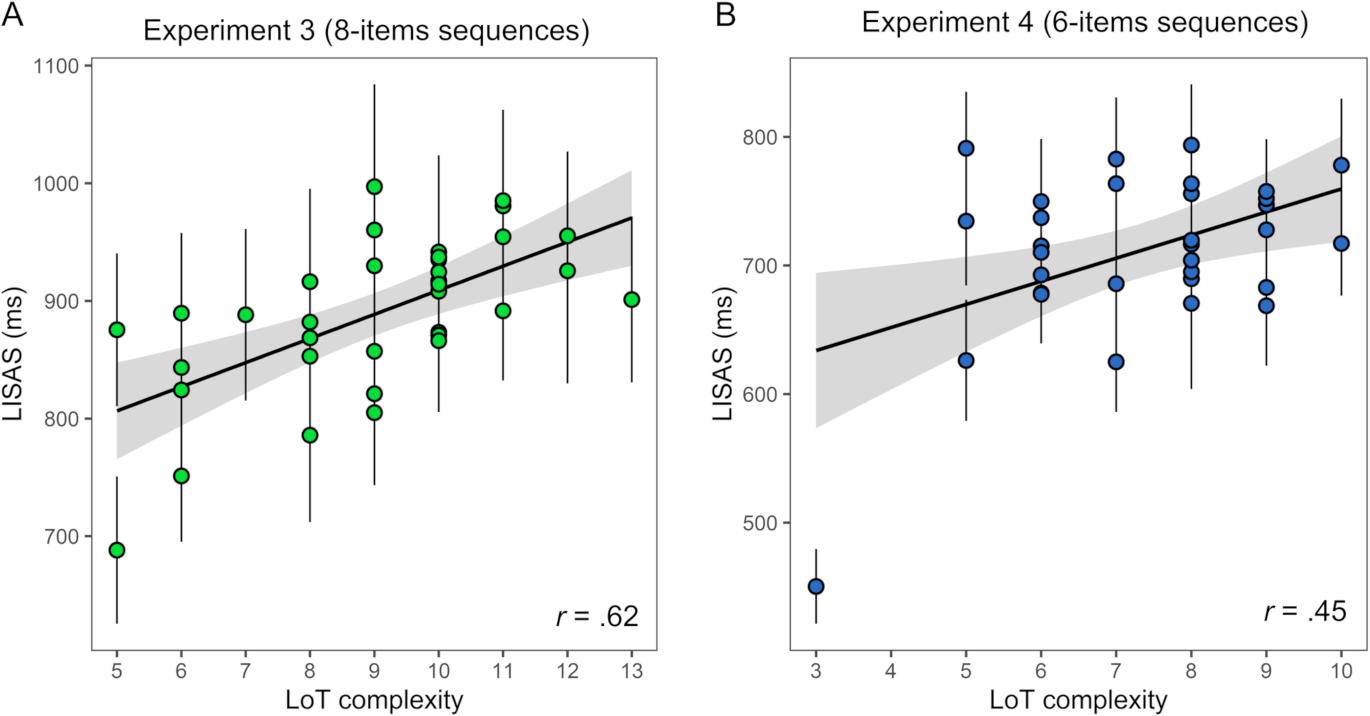
\includegraphics[scale=1]{journal.pcbi.1008598.g006.PNG}
      \centering
      %Linear relationship between LoT complexity and violation detection task performance (LISAS) in: (A) experiment 3 (8-items sequences) and (B) experiment 4 (6-items sequences).
      \caption{Relación lineal entre la complejidad LoT y el desempeño de la tarea de detección de violaciones (LISAS) en: (A) Experimento 3 (secuencias de 8 elementos) y (B) Experimento 4 (secuencias de 6 elementos)}
      \label{PlosBIO-F6}
\end{figure}
\sergio{la figura no está traducida}

\subsection{Experimento 5: secuencias auditivas y visuales}

%The observation of a LoT complexity effect on sequences of length 8 and higher is consistent with our initial claim that individuals spontaneously apply simple rules (mainly based on nested repetitions) in order to recode auditory sequences in a compressed abstract form in memory. It may be argued, however, that rather than being abstract and universal, some of these effects may reflect the great ability of our auditory system to manipulate and find regularities in acoustic stimuli (90); whether it is in spoken language or in music listening. In experiment 5, we wished to replicate the findings of previous experiment and extend them to the visual modality. Although we expected a reduced performance, given that audition is generally superior to vision in the processing of temporal information (91), we still predicted a correlation of performance with our complexity metric, since our language was originally designed for a visual paradigm (58) and relies on abstract mental operations rather than on specific acoustic coding mechanisms. Twelve sequences of 8 items (see Fig. S7), allowing to use a sufficient number of trials while still expecting clear complexity effects, were presented to a group of participants in both a visual and in an auditory form (in different experimental blocks), using the same violation detection paradigm. Due to constraints in the perception of repeated visual stimuli, stimulus onset asynchrony was lengthened to 400 ms in both auditory and visual sessions, resulting in a sequence duration of 3000 ms (compared to 1800 ms in experiment 2).

La observación de un efecto de la complejidad LoT en secuencias de longitud 8 y superior es consistente con nuestro planteo inicial de que los individuos espontáneamente aplican reglas simples (basada principalmente en repeticiones anidados ) con el fin de recodificar secuencias auditivas en una forma abstracta más comprimido en la memoria. Sin embargo, se puede argumentar que -en lugar de ser abstractos y universales- algunos de estos efectos pueden reflejar la gran capacidad de nuestro sistema auditivo para manipular y encontrar regularidades en los estímulos acústicos (\cite{f90}); ya sea en el lenguaje hablado o escuchando música. En el experimento 5, deseamos replicar los hallazgos del experimento anterior y extenderlos a una modalidad visual. A pesar de que esperábamos un rendimiento reducido (dado que la audición es generalmente superior a la visión en el procesamiento de información temporal (\cite{f91})) todavía esperamos encontrar una correlación del rendimiento con nuestra métrica de complejidad, ya que nuestro lenguaje fue diseñado originalmente para un paradigma visual (\cite{amalric2017language}) y se basa en operaciones mentales abstractas más que en mecanismos de codificación acústica específicos. Se presentaron a un grupo de participantes doce secuencias de 8 elementos (ver Figura~\ref{PlosBIO-S7}) tanto en forma visual como auditiva (en diferentes bloques experimentales), utilizando el mismo paradigma de detección de violaciones. Debido a las limitaciones en la percepción de estímulos visuales repetidos, la asincronía inicio de estímulo se alargó a 400ms en ambas sesiones (auditivas y visuales), lo que resulta en una duración de la secuencia de 3000ms (en comparación con 1800ms en el experimento 2).

\subsubsection{Efectos de complejidad y modalidad}

%To assess the impact of LoT complexity and modality on performance, we first estimated a mixed model including complexity and modality as fixed factors and participants as a random factor. Effects of LoT complexity (t(486.0) = 3.08, p = .003), modality (average LISAS of 1110 ms in visual blocks vs. 780 ms in auditory blocks; t(486.0) = 14.1, p < .0001) and their interaction (t(486.0) = 3.19, p = .002) were significant. The slope of the complexity effect was steeper in the visual than in the auditory modality (+54 ms vs. +22 ms, t(486) = 3.19; see Figure 7, and Fig. S8). Separate analyses indicated that LoT complexity was a strong predictor of performance for visual sequences (t(233.0) = 6.82, p < .0001; r = .76), and also for auditory sequences (t(237.0) = 3.76, p < .001; r = .63).

Para evaluar el impacto de la complejidad y la modalidad de LoT en el rendimiento, primero estimamos un modelo mixto que incluye la complejidad y la modalidad como factores fijos y los participantes como un factor aleatorio. Efectos de la complejidad de LoT ( t ( 486.0) = 3.08, p = .003), modalidad (LISAS promedio de 1110 ms en bloques visuales vs 780 ms en bloques auditivos; t ( 486.0) = 14.1, p <.0001) y su interacción ( t ( 486.0) = 3.19, p< = 0,002) fueron significativas. La pendiente del efecto de complejidad fue más pronunciada en la modalidad visual que en la auditiva (+5 4 ms frente a +22 ms , t (486) = 3,19 ; ver Figura 7 y Figura S8 ). Análisis separados indicaron que Lot complejidad era un fuerte predictor de rendimiento para secuencias visuales ( t ( 233 . 0 ) = 6,82 , p <0,0001; r . = 76 ), y también para las secuencias auditivas ( t ( 237,0 ) = 3,76 , p <. 001; r = .63).

%Note that, although the effects appeared stronger in the visual modality, the average performance in the visual and the auditory modality were highly correlated (r = .85, p < .0001). This suggests a common, cross-modal mechanism underlying the observed differences in performance between sequences. It can however be acknowledged, here again, that differences in performance across sequences are not entirely explained by complexity: residuals of linear regressions with LoT complexity in the visual and in the auditory modality (using average LISAS per sequence) were correlated (r = .73, t(13) = 3.92; p = .002).

Nótese que, aunque los efectos parecían más fuertes en la modalidad visual, el desempeño promedio en la modalidad visual y auditiva estuvieron altamente correlacionados ($r = .85, p <.0001$). Esto sugiere un mecanismo común entre las modalidades subyacente a las diferencias observadas en el rendimiento entre secuencias. Sin embargo, se puede reconocer nuevamente que las diferencias en el rendimiento entre secuencias no se explican completamente por la complejidad: los residuos de regresiones lineales con la complejidad LoT en la modalidad visual y en la modalidad auditiva (usando LISAS promedio por secuencia) estaban correlacionados ($r =.73, t (13) = 3.92; p = .002$).

%The number of false alarms per sequence was related to the task modality (mean number of FA: 0.58 in auditory blocks; 1.16 in visual blocks; difference between modalities: t(487.0) = 5.73, p < .0001) but not to sequence LoT complexity (t(487.0) = 0.08, p = .935).

El número de falsas alarmas por secuencia se relacionó con la modalidad de la tarea (número medio de FA : 0.58 en bloques auditivos; 1.16 en bloques visuales; diferencia entre modalidades: $t ( 487.0 ) = 5.73 , p <0.0001$) pero no con la complejidad LoT ( $t( 487.0 ) = 0.08, p =.935$).

\begin{figure}[t!]
      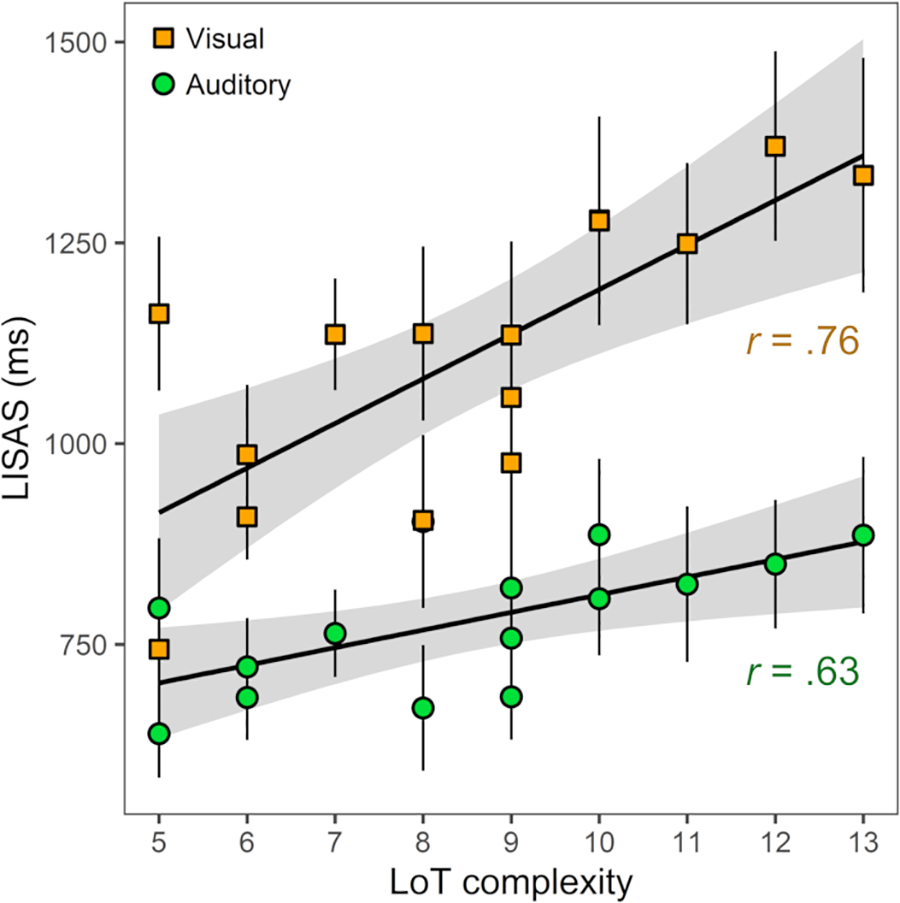
\includegraphics[scale=1]{journal.pcbi.1008598.g007.PNG}
      \centering
      % Linear relationship between LoT complexity and violation detection task performance (LISAS) for each modality in experiment 5 (8-items auditory and visual sequences).
      \caption{Relación lineal entre complejidad LoT y rendimiento en tareas de detección de violación (LISAS) para cada modalidad en experimento 5 (secuencias auditivas y visuales de 8 elementos)}
      \label{PlosBIO-F7}
\end{figure}
\sergio{la figura no está traducida}

\subsubsection{Efectos de sorpresa}

%As in previous experiments, a surprise effect was also observed in both modalities when considered independently: deviants inducing rare transitions were more easily and quickly detected than frequent ones (effect of surprise in a mixed model with auditory trials only: t(237.0) = 3.87, p < .001; r = –.65; with visual trials only: t(233.0) = 6.79, p < .0001; r = –.78). This effect suggests that a common, or at least similar, mechanism is at play in the encoding of statistical regularities characterizing the sequences in both the visual and the auditory modality. 

Como en los experimentos anteriores, también se observó un efecto sorpresa en ambas modalidades cuando se consideraron de forma independiente: las super-desviaciones que inducían transiciones raras se detectaban más fácil y rápidamente que las relacionadas a elementos frecuentes (efecto de sorpresa en un modelo mixto con pruebas auditivas solamente: $t(237.0) = 3.87, p <.001; r =- .65$; solo con pruebas visuales: $t (233.0) = 6.79, p <.0001; r = –.78$). Este efecto sugiere que un mecanismo común, o al menos similar, está en juego en la codificación de regularidades estadísticas que caracterizan las secuencias tanto en la modalidad visual como en la auditiva.

%In order to test whether evidence for sequence compression could still be observed after the surprise effect was taken into account, we performed a comparison of mixed effects models. The null model included the surprise predictor, the modality as a categorical predictor and subject identity as random factor. It was compared against a full model including the same predictors, with addition of the LoT complexity. This comparison was highly significant (χ²(1) = 19.0, p < .0001), indicating that goodness of fit improved when LoT complexity was added to the model. All three fixed effects were significant in the full model (LoT complexity: t(486.0) = 4.39, p < .0001; surprise: t(486.0) = 4.54, p < .0001; modality: t(486.0) = 14.2, p < .0001, see Table 1).

Para probar si aún se podía observar evidencia de compresión de secuencia después de que se tuvo en cuenta el efecto sorpresa, realizamos una comparación de modelos de efectos mixtos. El modelo nulo incluyó el predictor de la sorpresa, la modalidad como predictor de categoría y la identidad del sujeto como factor aleatorio. Se comparó con un modelo completo que incluía los mismos predictores, con la adición de la complejidad LoT. Esta comparación fue altamente significativa ($\chi^2 (1) = 19.0, p <.0001$), lo que indica que el ajuste mejoró cuando se agregó la complejidad LoT al modelo. Los tres efectos fijos fueron significativos en el modelo completo (complejidad LoT: $t (486.0) = 4.39, p <.0001$; sorpresa: $t (486.0) = 4.54, p <.0001$; modalidad: $t (486.0) = 14.2, p <0,0001$, ver Tabla~\ref{PlosBIO-T1}).

%Overall, the results obtained in the visual modality are very similar to those obtained in the auditory modality in the same and in previous experiments. We however observed here stronger effects of both LoT complexity and surprise. It should be noted that the overall difficulty of the task increased in the visual modality (as indicated by higher average miss rates per sequence; 22\% vs. 11\%, t(14) = 7.49, p < .0001; and longer average response times per sequence; 831 ms vs. 645 ms, t(14) = 10.5, p < .0001). 8-items visual sequences may have been more difficult to encode than 8-items auditory sequences, due to the known superiority of the auditory processing system in the processing of temporal sequences and rhythms (90,92). This increased encoding difficulty in the visual domain may have in turn lead to an increased need for the “mental sequence compression” mechanism that our language of thought aims to describe.

En general, los resultados obtenidos en la modalidad visual son muy similares a los obtenidos en la modalidad auditiva en el mismo experimento y en los anteriores. Sin embargo, observamos aquí efectos más fuertes tanto de la complejidad LoT como de la sorpresa. Hay que señalar que la dificultad general de la tarea aumenta en la modalidad visual (como se indica por el aumento promedio de las tasas de error por secuencia; 22\% vs. 11 \% , $t (14) = 7.49, p <0.0001$; y del tiempo medio de respuesta por secuencia; 831ms frente a 645ms, $t(14) = 10.5, p <0.0001$). En las secuencias visuales de 8 elementos pueden haber sido más difíciles de codificar que las secuencias auditivas de 8 elementos, debido a la superioridad conocida del sistema auditivo para el procesamiento de secuencias temporales y ritmos \cite{f90,f92}. Esta mayor dificultad de codificación en el dominio visual puede, a su vez, llevar a una mayor necesidad de utilizar el mecanismo de ``compresión de la secuencia mental'' que nuestro LoT pretende describir.

%The present experiment also extends the results of experiment 3 by using a slower presentation rate. Indeed, although the participants in experiment 5 appeared to respond faster (in the auditory blocks) than those from experiment 3, the same relationship with complexity was found (correlation of performance with LoT complexity of .62 and .63 respectively). It suggests that the effect of complexity is robust across sequence durations (as expected given than LoT complexity is based on abstract sequence patterns). More importantly, the fact that a similar complexity effect was observed irrespective of the modality is consistent with the idea of “language of thought” used to compress sequential information at an abstract, symbolic level. Such an assumption has already been supported by results from Yildirim and Jacobs (93), who showed cross-modal transfer of sequence knowledge: learning to categorize visual sequences facilitated the categorization of auditory sequences and vice versa. In fact, the language we used here was initially designed to represent visually presented, geometrical patterns (58). The present results thus confirm that the present language of thought can account for sequence representations in various modalities, presentation contexts and sequence lengths.

El presente experimento extiende también los resultados del experimento 3 utilizando una tasa de presentación más lenta. De hecho, aunque los participantes del experimento 5 parecían responder más rápido (en los bloques auditivas) que los del experimento 3, se encontró la misma relación con la complejidad LoT (correlación de rendimiento con complejidad LoT de 0,62 y 0,63, respectivamente). Esto sugiere que el efecto de la complejidad es robusto a través de la duración de las secuencias (como se esperaba dado que la complejidad LoT se basa en patrones de secuencias abstractos). Más importante aún, el hecho de que se observó un efecto de complejidad similar independientemente de la modalidad es consistente con la idea de un ``lenguaje de pensamiento'' (LoT) utilizado para comprimir información secuencial a un nivel simbólico abstracto. Tal suposición se apoya también en los resultados de Yildirim y Jacobs \cite{yildirim2015learning}, que mostraron efectos de transferencia de aprendizaje entre modalidades de las secuencias: aprender a categorizar secuencias visuales facilitó la categorización de secuencias auditivas y viceversa. De hecho, el lenguaje que usamos aquí fue inicialmente diseñado para representar patrones geométricos presentados de manera visual \cite{amalric2017language}. Los presentes resultados confirman así que el lenguaje actual del pensamiento puede dar cuenta de las representaciones de secuencia en diversas modalidades, contextos de presentación y longitudes de secuencias.

\subsection{Análisis adicional: comparación con otras medidas de complejidad de secuencias}

\section{Discusión General}

\section{Materiales y métodos}
\sergio{Pasar a suplemento}

%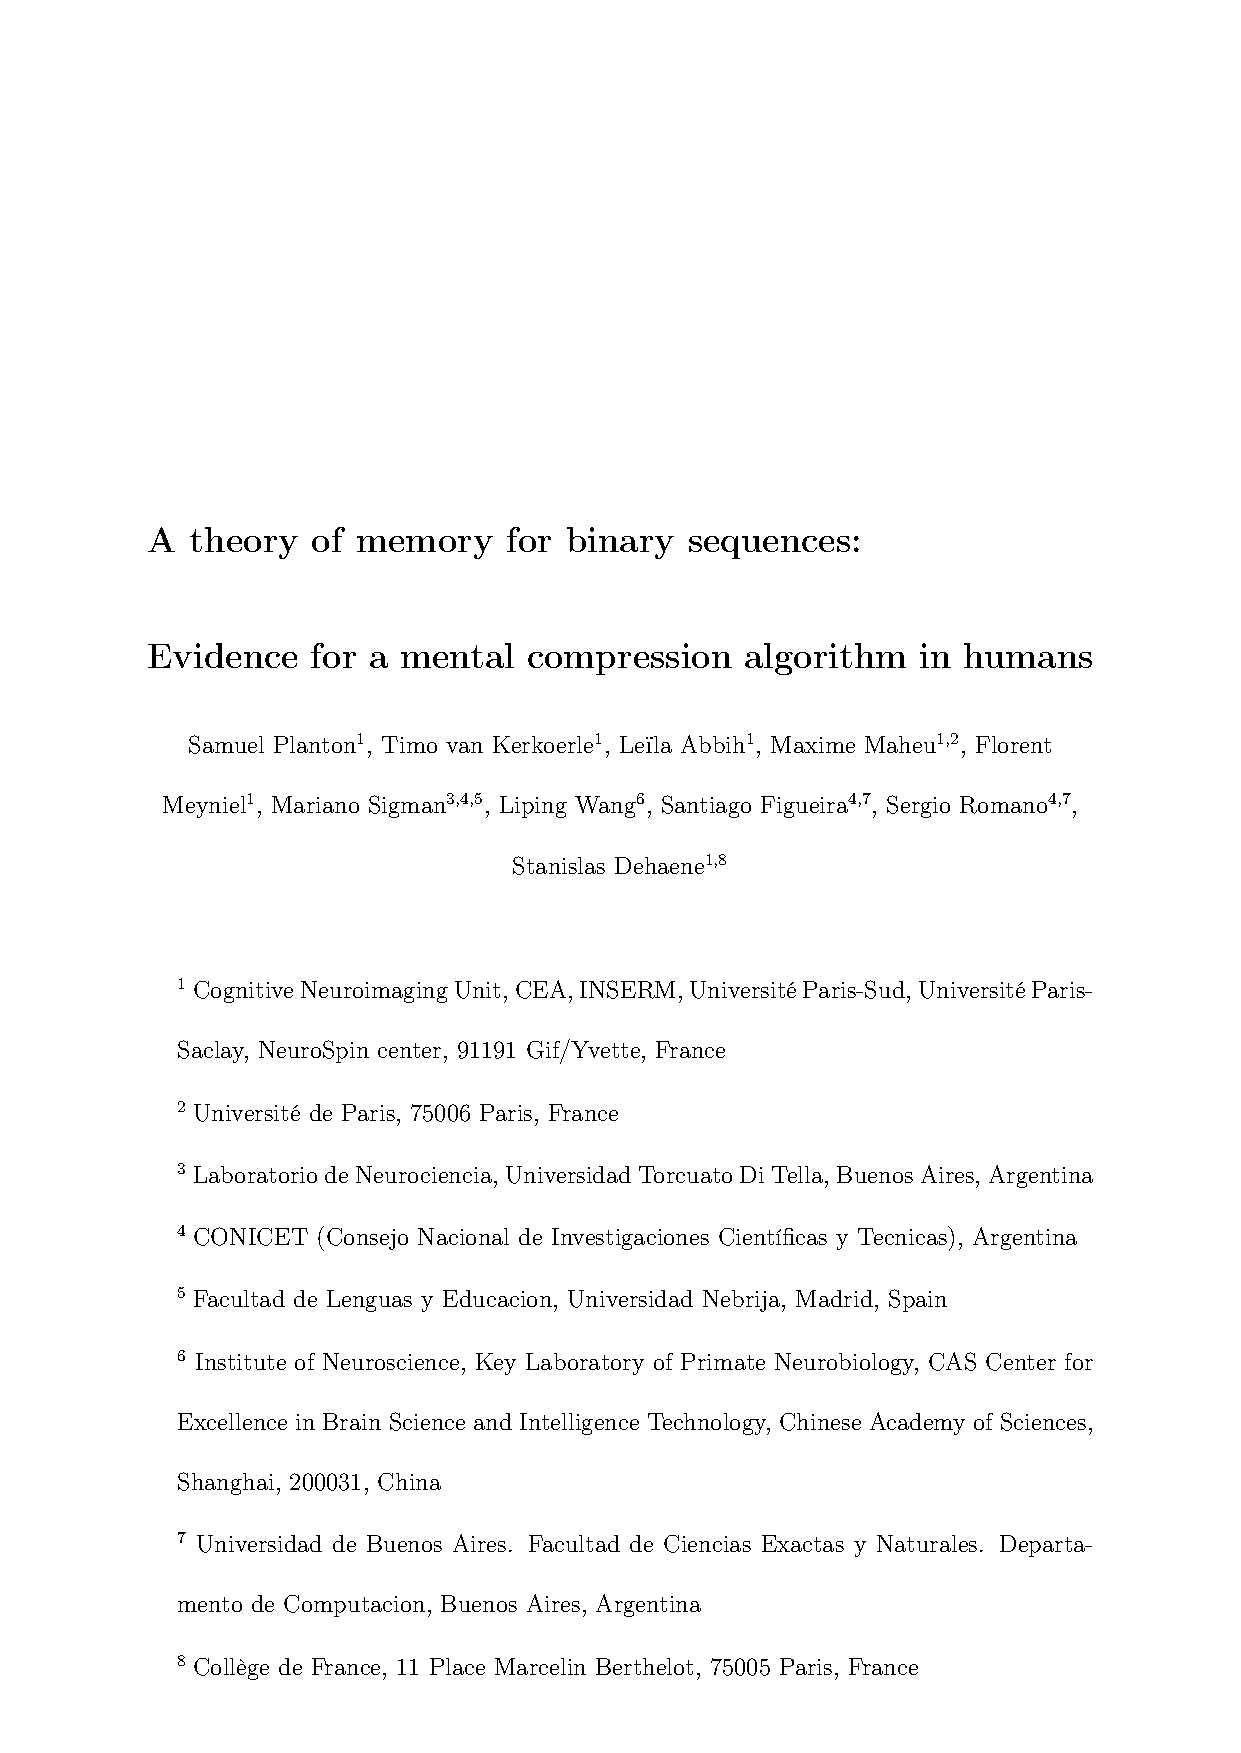
\includepdf[pages=-]{manuscript_pcb.pdf}